\documentclass{article}

\usepackage{siunitx} % Provides the \SI{}{} and \si{} command for typesetting SI units

\usepackage{graphicx} % Required for the inclusion of images

\usepackage{tabularx} % Tables

\usepackage{natbib} % Required to change bibliography style to APA

\usepackage{amsmath} % Required for some math elements

% Many options for pseudocode
\usepackage{algorithm}
\usepackage{algpseudocode}

%side by side figures
\usepackage{caption}
\usepackage{subcaption}

\usepackage{listings} % Python code blocks

\usepackage{comment}

\usepackage[left=1in,top=1in,bottom=1in,right=1in]{geometry}

\setlength\parindent{0pt} % Removes all indentation from paragraphs

\title{Lab \#6 Report: Path Planning} % Title

\author{Team \#4 \\\\ Frank Gonzalez \\ Marisa Hoosen \\ Toomas Tennisberg \\ Zoe Wong \\ Kaitlin Zareno \\\\ RSS} % Team # + Names, Class (RSS)

\date{\today} % Date for the report

\begin{document}

\maketitle

\begin{comment}
(no more than 4500 words total, not including Lessons Learned; each team member should contribute approximately equal amounts to the writing of this report)\\
\end{comment}

\section{Introduction}
Written by: Toomas Tennisberg\\\\
Path planning is an important component for our racecar. Not only is it useful for high level autonomous navigation, it is a critical component for the city navigation aspect of the final challenge. Therefore, we added RRT and Pure Pursuit to the localization solution we developed in the previous lab to teach the robot how to determine and follow a path from point A to point B.\\\\
The goal of this lab was to get path planning working, both in simulation and on the racecar itself. Specifically, we want to have a path planning algorithm that finds a path to the destination, ideally within a few seconds, and a path following algorithm that does not stray far from a given path. We tested both solutions separately in simulation by manually observing the results of a few cases, as well as submitting them for automated unit testing. We also tested the fusion of the two solutions manually, both in simulation and real life.\\\\
Path planning is complicated to achieve in real life. Our main concerns were getting our path planning algorithms to converge on a solution in less than a minute and making sure pure pursuit stays on the given path. In the next sections, we explain the exact details of how our solution works.

\section{Technical Approach}

\subsection{Path Planning}
\subsubsection{RRT Algorithm}
Written by Frank Gonzalez and Katelin Zareno\\

The first path planning algorithm we implemented was a rapidly-exploring random tree (RRT). RRT constructs a graph out of a space by randomly sampling points and connecting them in a strategic manner. The algorithm requires an initialization for the car's pose, a position for the goal, and a map that describes where obstacles are located throughout the environment. The pseudocode for RRT is provided below:
\pagebreak

\begin{algorithm}
\caption{RRT (Start, Goal, Map)}\label{alg:cap}
\begin{algorithmic}[1]
\State $path\_found$ = False
\State $free\_{uv}$ = initialize\_uv\_space()
\State $valid\_states$ = \{Start\}
\While{not $path\_found$}
    \State $uv$ = get\_free\_uv()
    \State $xy$ = to\_xy($uv$)
    \State $nearest$ = get\_closest($valid\_states$)
    \State $new\_xy$ = step($nearest$, $xy$, $step\_dist$)
    \If{collision($nearest$, $new\_xy$, Map)}
        continue
    \EndIf
    \State $valid\_states$ $\cup$ $new\_xy$
    \If {near\_goal($new\_xy$, Goal, $tolerance$)}
        make\_path($new\_xy$)
    \EndIf
\EndWhile
\end{algorithmic}
\end{algorithm}

The algorithm begins by initializing a free $uv$ space. U, v space is the same pixel space in which the occupancy map of the environment is provided. The occupancy map provides information as to whether or not a certain location is blocked by an obstacle, so working in the $uv$ space provides a natural way to sample the free space. The occupancy map also provides the following information: a scaling factor to match the map scale to the real world scale, and a transformation including a rotation and translation to match the origins of the map and real world environment. The latter two bits of information are encoded in the following matrix:

\begin{equation}
   transformation = \begin{bmatrix} \cos(\theta) & -\sin(\theta) & 0\\ \sin(\theta) & \cos(\theta) & 0  \\ 0 & 0 & 1\end{bmatrix}
\end{equation}

Additionally, the algorithm initializes the set $valid$ which will contain all of the nodes that have been added to the tree. Each node will be an instance of a class called SearchNode, which is outlined below:
% \pagebreak

\begin{lstlisting}
class SearchNode(object):
    def __init__(self, parent=None, location):
        self.location = location
        self.parent = parent
    
    def dist(self, other):
        return euclidean distance
      
    def get_vec(self, other):
        return unit_vec
\end{lstlisting}

This representation of a tree node is useful because it allows us to establish parent pointers as well as get the relationship between one node and another. The parent pointers will make extracting a path easier while the unit vector and distance function help find new nodes and determine where to place them within the tree.\\

The algorithm begins random sampling by first converting a sampled $uv$ point into an $xy$ point. This transformation occurs as follows:

\begin{equation}
    \begin{bmatrix}x \\ y \\ z \\ 1 \end{bmatrix} = \begin{bmatrix} transformation & map\_pos \\ 0 & 1 \end{bmatrix}\begin{bmatrix} resolution*v \\ resolution*u \\ 0 \\ 1 \end{bmatrix}
\end{equation}

It then determines which node in $valid$ is closest to this sampled point by using the dist function from SearchNode. Then, the algorithm steps in the direction of the sampled point, from the closest tree node, by distance d, which in our algorithm was set to 0.5 {m}.\\

Next, the algorithm must check for collision between the closest tree node and the new location. A small pseudocode is provided for this check:

\begin{algorithm}
\caption{collision (nearest, new\_xy, Map)}\label{alg:cap}
\begin{algorithmic}[1]
\State $collision$ = False
\State $step$ = d/10
\State $cur$ = nearest
\State $unit_vec$ = nearest.get\_vec(new\_xy)
\While{dist($cur$, new\_xy) $>$ step and not $collision$}
    \State $cur$ = $cur$ + $unit\_vec$*$step$
    \State $cur\_pixels$ = to\_pixels($cur$)
    \State $collision$ = not Map[$cur\_pixels$] == free
\EndWhile
\State return $collision$
\end{algorithmic}
\end{algorithm}

The collision algorithm steps from the closest node in the tree towards new\_xy, checking for obstacles at each intermediate position. Should a free path exist between the tree and new\_xy, a SearchNode instance is created with a parent pointer directed towards $closest$. This process then continues until a point in space is connected to the tree within some tolerance $tol$, which we set to 0.75 {m}. Once this condition is satisfied, a path is extracted by following the parent pointers of the final node.\\

\subsubsection{A*}
Written by: Frank Gonzalez and Kaitlin Zareno\\

The second path planning algorithm we implemented was A*. In A*, we create partial paths with an associated value that characterizes how good the path is via the following heuristic function: $f = g + h$, where $g$ represents the current accumulated cost of the path (i.e. how long the path is) and h represents an estimate for how much longer the path will become (the euclidean distance from the partial path's end to the goal). A*'s pseudocode is the following:

\begin{algorithm}
\caption{A* (Start, Goal, Map)}\label{alg:cap}
\begin{algorithmic}[1]
\State $priority\_queue$ = [([Start], 0, dist\_to\_goal(Start, Goal))]
\State $Visited$ = {Start}
\State $path\_found$ = False
\While{not $path\_found$ and len($priority\_queue$) != 0}
    \State $best$ = $priority\_queue$.pop()
    \If{at\_goal($best$)}
        make\_path($best$)
        path\_found = True
    \EndIf
    \State $new\_neighbors$ = get\_neighbors($best$, $Visited$)
    \For {neighbors in $new\_neighbors$}
        \State $partial\_path$ = make\_partial\_path($best$, neighbor)
        \State $new\_cost$ = $best$[old\_cost] + dist($best$[final\_node], neighbor)
        \State $estimate$ = dist(neighbor, Goal)
        \State $Visited$ $\cup$ neighbor
        \State $priority\_queue$.append([(partial\_path, $new\_cost$, $estimate$)])
    \EndFor
    \State $priority\_queue$.sort()
\EndWhile

\end{algorithmic}
\end{algorithm}
The algorithm begins by initializing a queue. The elements in the queue are sorted in decreasing order according to the heuristic, such that the element with the smallest heuristic value exists at the end of the list and the element with the largest heuristic value exists at the beginning of the list. Furthermore, each element in the queue is a tuple of a sequential list of nodes that represent the current path, the length of the current path from the start node to the current node (as defined above by the value, g), and the distance from the current node to the goal node (as defined above by the value, h). Like in the RRT algorithm defined above, each node is represented as an object in the SearchNode class, and contains information regarding a node's parent and location. Once we have our queue, we then begin iteration. Pulling the "best" node (node with smallest heuristic value) from the queue, we first check if the node exists at the target location. If the target location has been found, we then backtrack from the current node (destination) to the start node using parent pointers to reconstruct the path. If a path is not found, we obtain the neighbors of the current node, as defined by the 8 nodes that border the current node in 2D pixel space, if they have not already been visited. If a neighbor node can help create a more optimal path, we add it to the queue in the format described above. Once all these neighbors have been added to the queue, we re-sort the queue based on the heuristic and repeat the process until we've found a path.\\   

\subsection{Path Planning Evaluation}
Written By: Kaitlin Zareno\\

In the path planning evaluation section, we will define our algorithm comparison criteria, the reasoning for implementing a specific search algorithm, and the effects of map data preprocessing on our comparison criteria. 

\subsubsection{RRT vs. A*}
In order to evaluate the success of our algorithms, we will compare the time of convergence for RRT and A* across maps that have different erosion factors (0.5, 0.6, 0.7, & 0.8) and different expected optimal trajectories. The times of convergence and generated paths for a straight trajectory using RRT and A* are shown in the table and figure below.

\begin{table}[ht]
    \centering
    \begin{tabular}{|l|l|l|l|l|}
        \hline
        & 0.5 & 0.6 & 0.7 & 0.8\\\hline
        RRT & 1.326 & 2.404 & 3.562 & 0.813 \\\hline
        A* & 5.796 & 5.375 & 5.465 & 6.582\\ \hline
    \end{tabular}
    \caption{Straight Line Trajectory Convergence Times for RRT and A*\label{BACtable}}
\end{table}

\begin{figure}[h]
\begin{center}
\begin{tabular}{c|c}
    RRT & A* \\
    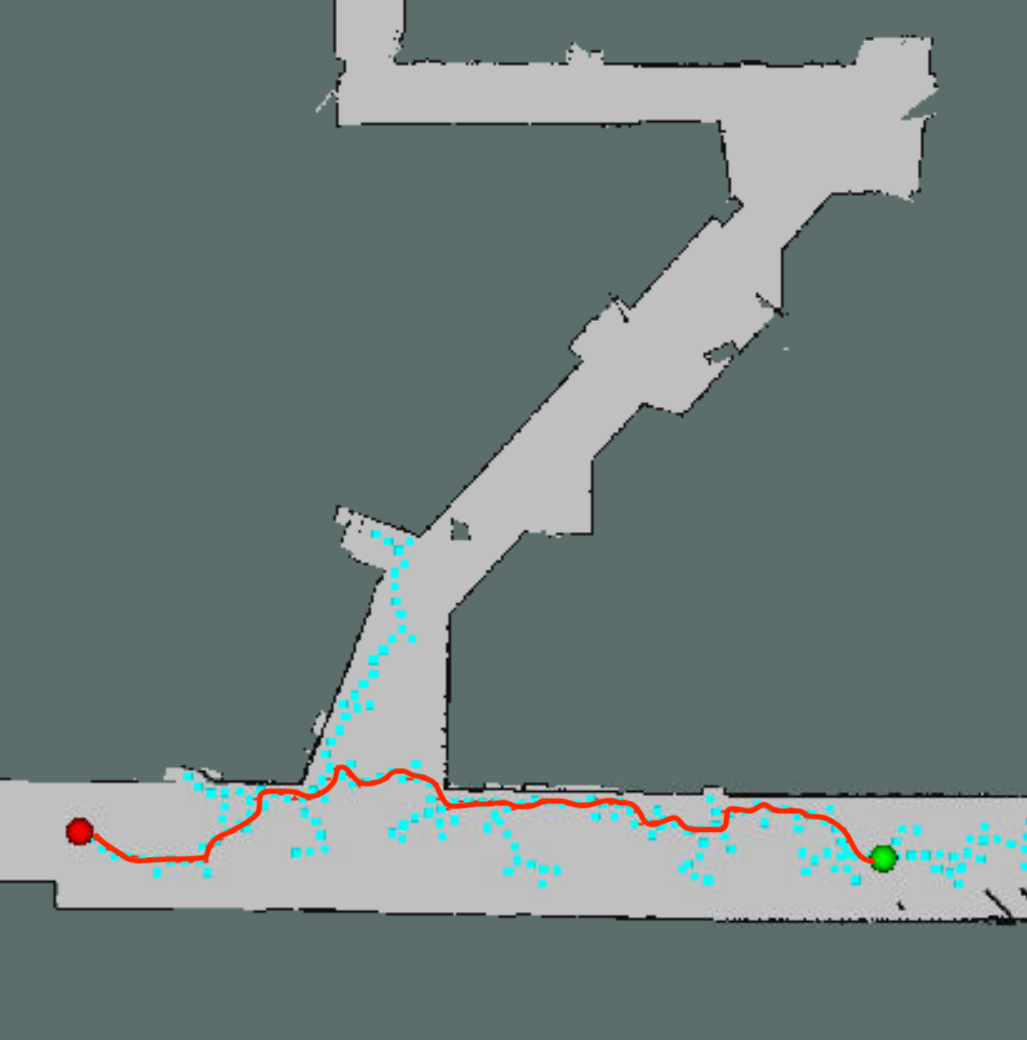
\includegraphics[scale=.5]{RRT-Straight.png} & 
    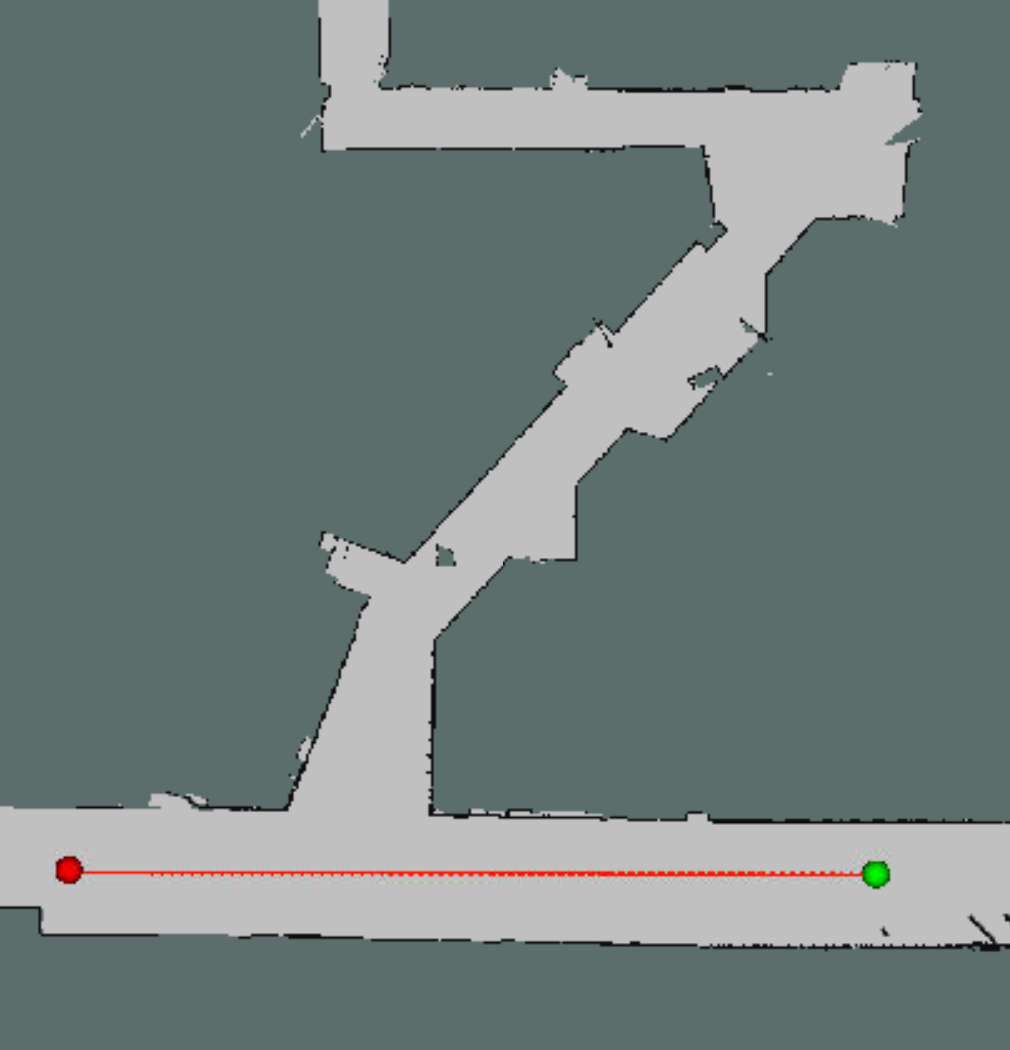
\includegraphics[scale=.5]{A_Star_Straight.png} & 
\end{tabular}
\caption{RRT vs A* Straight Trajectory Comparison}
\end{center}
\end{figure} 

According to Table 1 above, we can see that RRT outperforms A* across all erosion values when trying to determine a straight line trajectory through open space. Since we're running a path planning algorithm through open space, the erosion factor will not affect RRT's ability to converge on a near optimal path from the start location to the desired end location. One reason why RRT may be performing so well in this situation is because of the difference in step-size. RRT has a default step size of 0.5 {m}, which spans multiple pixels, whereas A* must step pixel by pixel as it branches out. In addition, although RRT has a faster rate of convergence than A*, the proposed RRT path is more noisy and less optimal than the straight line path generated by A* due to the random-sampling aspect of the RRT algorithm. \\ The times of convergence and generated paths for the Gradescope trajectory using RRT and A* are shown in the table and figure below.

\begin{table}[ht]
    \centering
    \begin{tabular}{|l|l|l|l|l|}
        \hline
        & 0.5 & 0.6 & 0.7 & 0.8\\\hline
        RRT & 33.716 & 29.106 & 47.244 & 50.09 \\\hline
        A* & 10.152 & 9.85 & 9.36 & 8.293 \\ \hline
    \end{tabular}
    \caption{Gradescope Trajectory Convergence Times for RRT and A*\label{BACtable}}
\end{table}

\begin{figure}[h]
\begin{center}
\begin{tabular}{c|c}
    RRT & A* \\
    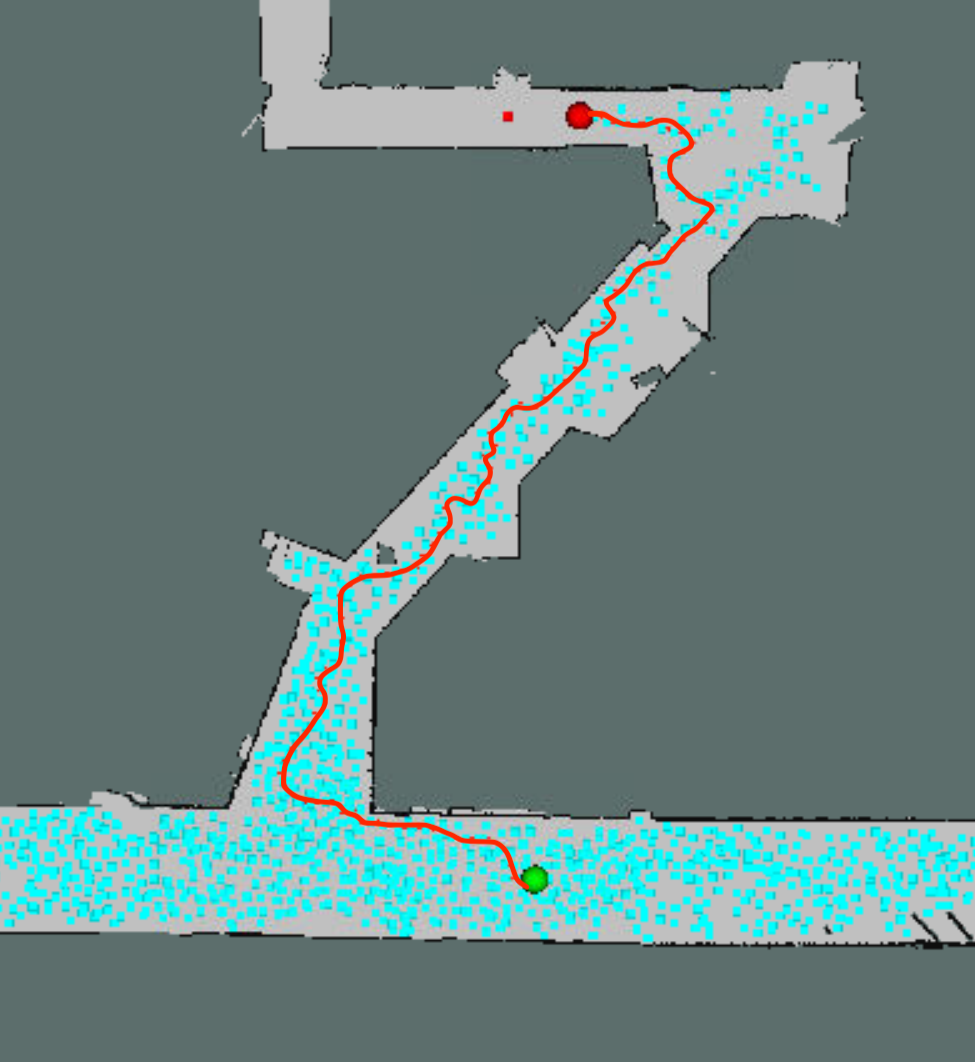
\includegraphics[scale=.5]{RRT-Gradescope.png} & 
    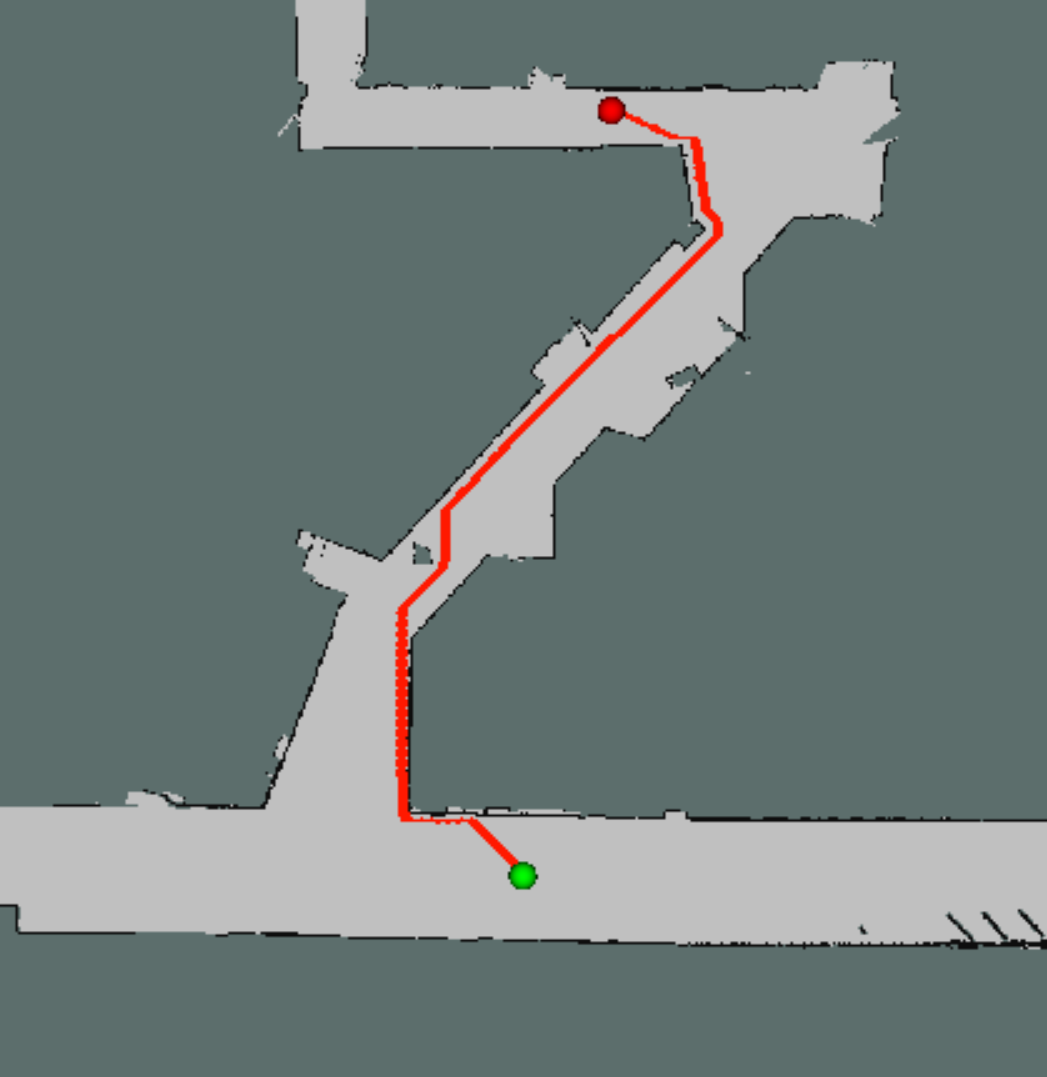
\includegraphics[scale=.5]{A_Star_Gradescope.png} & 
\end{tabular}
\caption{RRT vs A* Straight Trajectory Comparison}
\end{center}
\end{figure}
\\

According to table 2 above, A* outperforms RRT across all erosion values when trying to determine the Gradescope trajectory. This trajectory features 2 turns (one right turn and one left turn) as well as a column obstruction that decreases the width of one of the corridors. In this trajectory, erosion plays a role in each algorithm's ability to find a near-optimal path from the start location to end location. Since RRT is a sampling based algorithm, greater erosion will affect the probability of obtaining a line segment that experiences no collisions when obstacles exist in areas that already have a limited valid search space, and we will further discuss the effects of map pre-processing on RRT convergence in section 2.2.2 of the report. On the other hand, since A* is a search-based algorithm and creates connections based off valid neighboring nodes, it is able to find a near-optimal path from the start node to the end node regardless of how little free space there seems to be in the traversed corridors of the optimal trajectory, given that a path exists. \\

Furthermore, we can see that as the erosion factor increases, A* performs better—this may be due to the fact that we need to perform fewer calculations: a pixel surrounded by free space requires at most 8 values to be added to the queue, but a pixel that exists next to a boundary only requires at most 5 values to be added to the queue. Thus, if we increase the size of the boundary line, we're decreasing the number of nodes that will be sorted and iterated over. Lastly, we can see that although our implementation of A* does not give a fully optimal path, it still gives a near-optimal trajectory. \\

Although A* does not find a path as quickly as RRT when trying to create a straight trajectory in open space and RRT tends to find trajectories that decrease the risk of the car crashing into the walls due to valid paths being generated more centrally in corridors, it is more robust to finding a near-optimal path that adheres to the specifications given within a short time frame. Furthermore, since A* performs well with larger erosion values, if the erosion value is large enough, a planned trajectory that is flush with a boundary still won't cause the car to crash into the wall. Thus, since the search space in which we seek to create a path tends to include multiple turns and tight corridors and smaller convergence times are preferred, we proceeded with choosing A* as our motion planning algorithm for this lab. 

\subsubsection{Effects of Map Prepossessing on RRT Convergence} 
Map pre-processing defines the process in which the occupancy grid that represents our map is eroded. By eroding the map, we increase the width of the "boundaries;" this makes sure that algorithm planned path trajectories that are flush with the wall won't cause the robot to crash in real life or simulation. That said, increasing the width of the bounding lines causes thin corridors in our original representation to be even thinner, and this poses problems for our sampling-based algorithm, RRT. As mentioned above, larger eroding affects the probability of obtaining a line segment that experiences no collisions when obstacles exist in areas that already have a limited valid search space, as erosion will cause the valid search space to shrink even more. Thus, increasing the erosion makes it extremely hard for RRT to squeeze through narrow passageways, and increases the likelihood of RRT creating a convoluted, longer path that's easier to find in order to avoid the narrow corridors, even if traversing the narrow corridors would lead to a more optimal path. In the image below we can observe this phenomenon. We can see that RRT was unable to find a connection through the corridor, and instead chose to create a longer path through corridors with more open space.

\begin{figure}[h]
\begin{center}
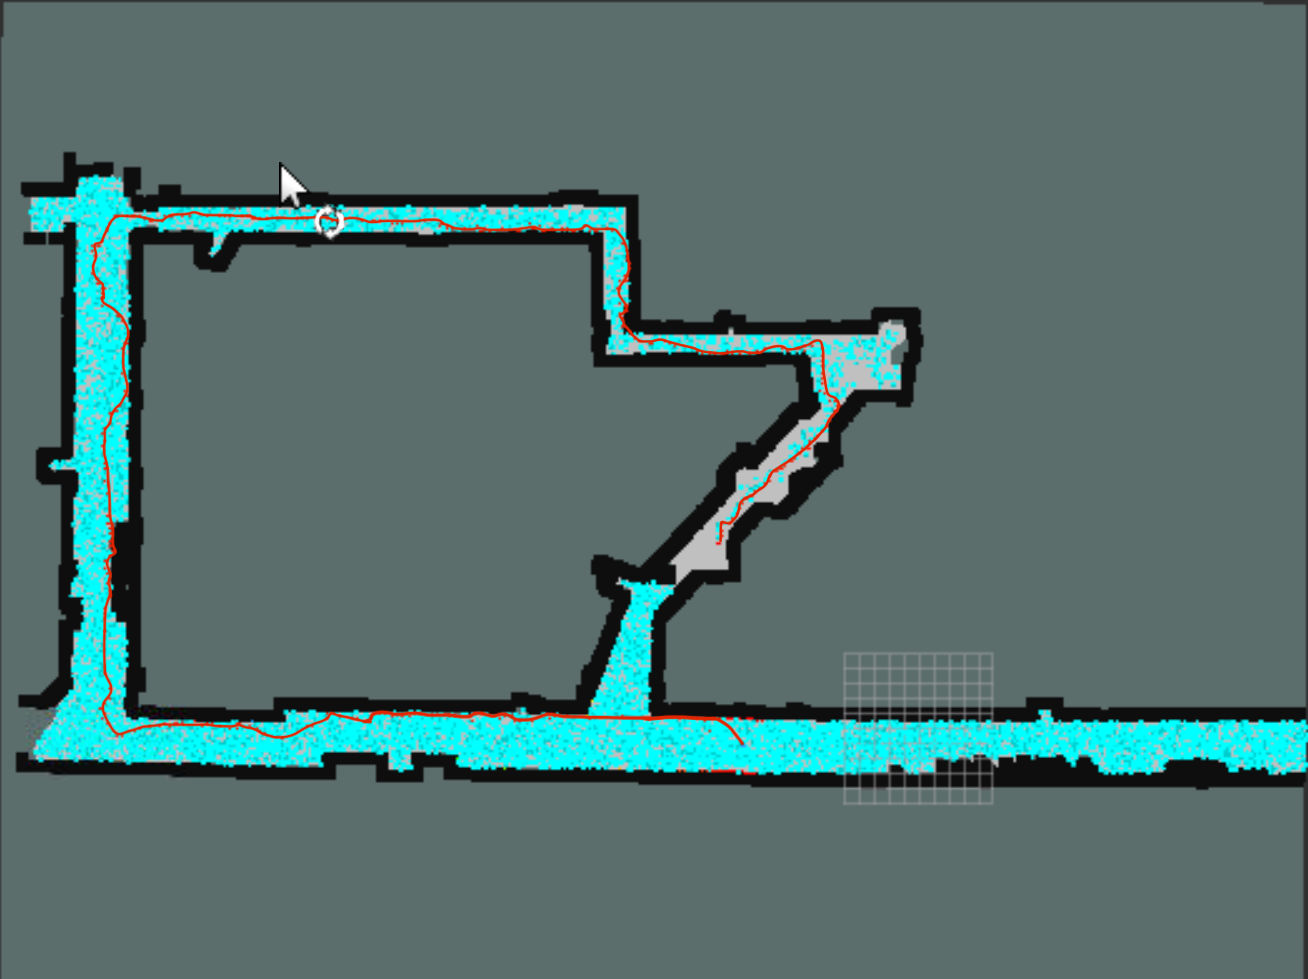
\includegraphics[width=0.5\textwidth]{convoluted_rrt.png}
\caption{RRT with Large Map Erosion}
\end{center}
\end{figure}

Thus, with increased erosion, RRT is less likely to find a path through the narrow passageway, and we typically observe the algorithm taking longer to converge, as displayed in Table 2.

\subsection{Pure Pursuit}
Written by: Marisa Hoosen and Toomas Tennisberg\\\\
Pure pursuit is a method of calculating the curvature of a vehicle to follow a given path. This consists of finding the closest (unvisited) segment to the robot, calculating the point on the segment closest to the robot using a bounding circle, and calculating the steering angle to the target point.

\subsubsection{Finding closest segment}
We find the closest segment by iterating over all segments in the trajectory and finding the minimum perpendicular distance to the robot. Figures 4a and 4b illustrate the robot choosing the closest segment that the robot has not yet tracked.\\

\begin{figure}[h]
    \centering
    \begin{subfigure}[b]{0.25\textwidth}
        \centering
        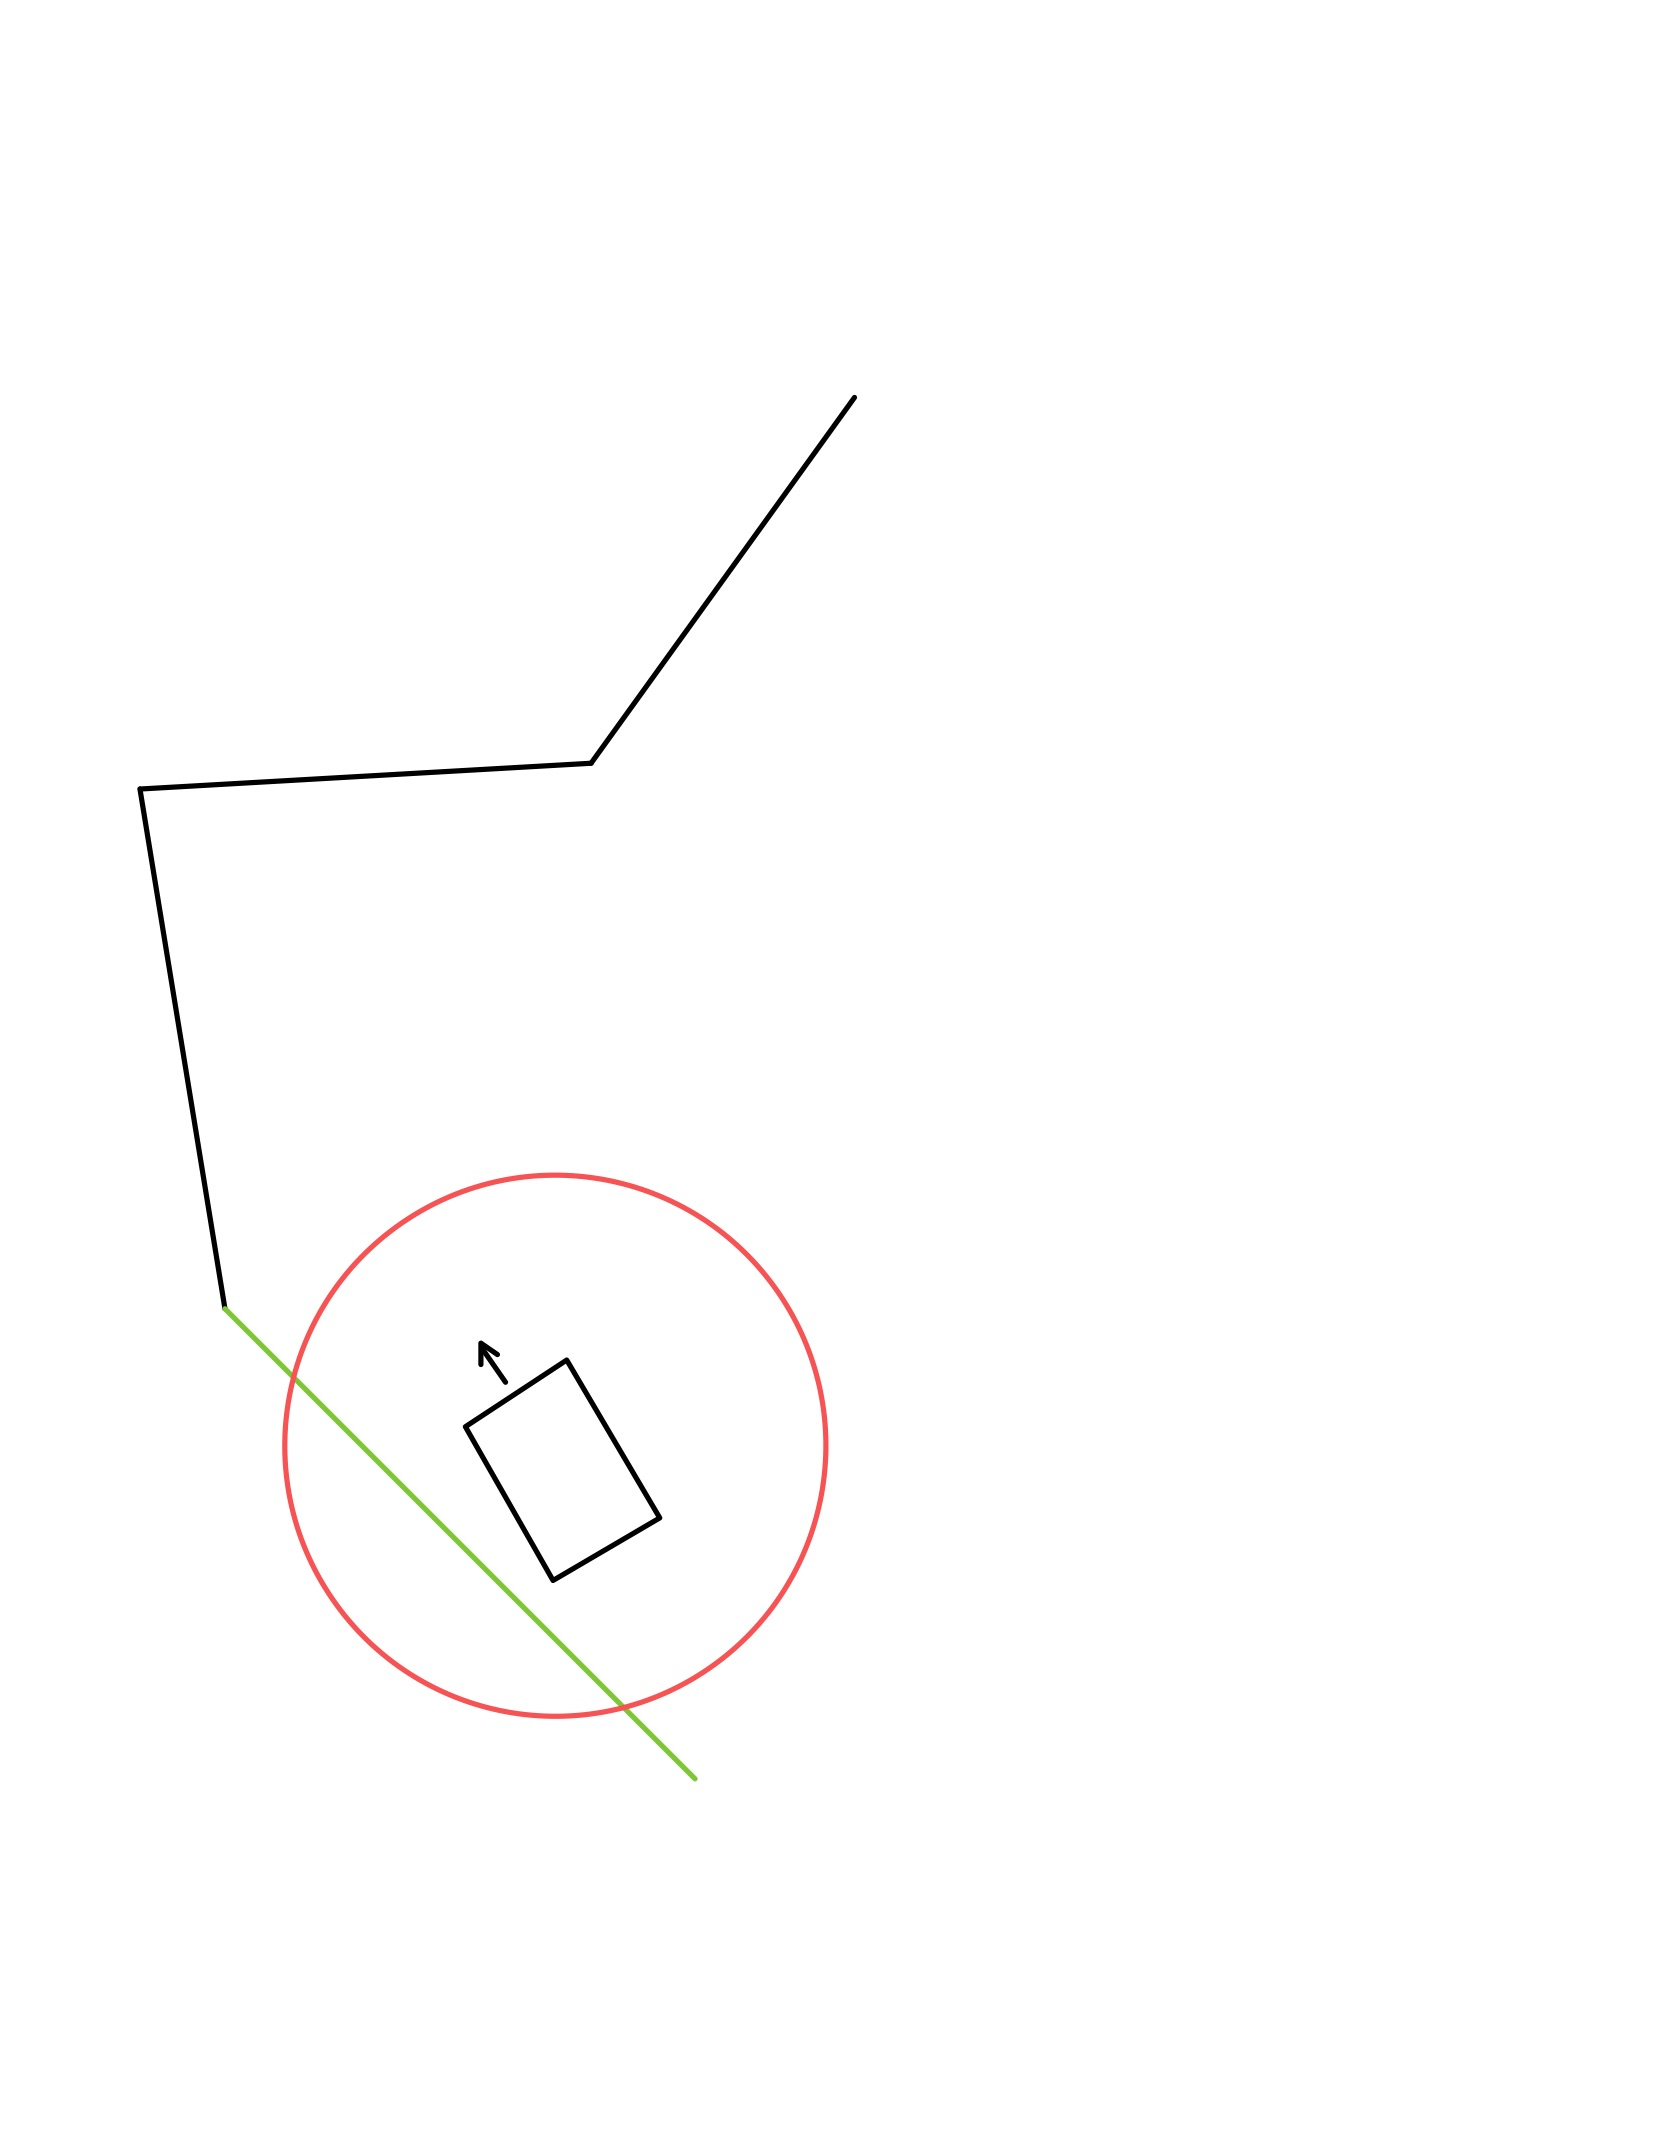
\includegraphics[width=\textwidth]{6.141-52.jpg}
        \caption{Closest segment to robot (green) and bounding circle (red)}
    \end{subfigure}
    \hfill
    \begin{subfigure}[b]{0.25\textwidth}
        \centering
        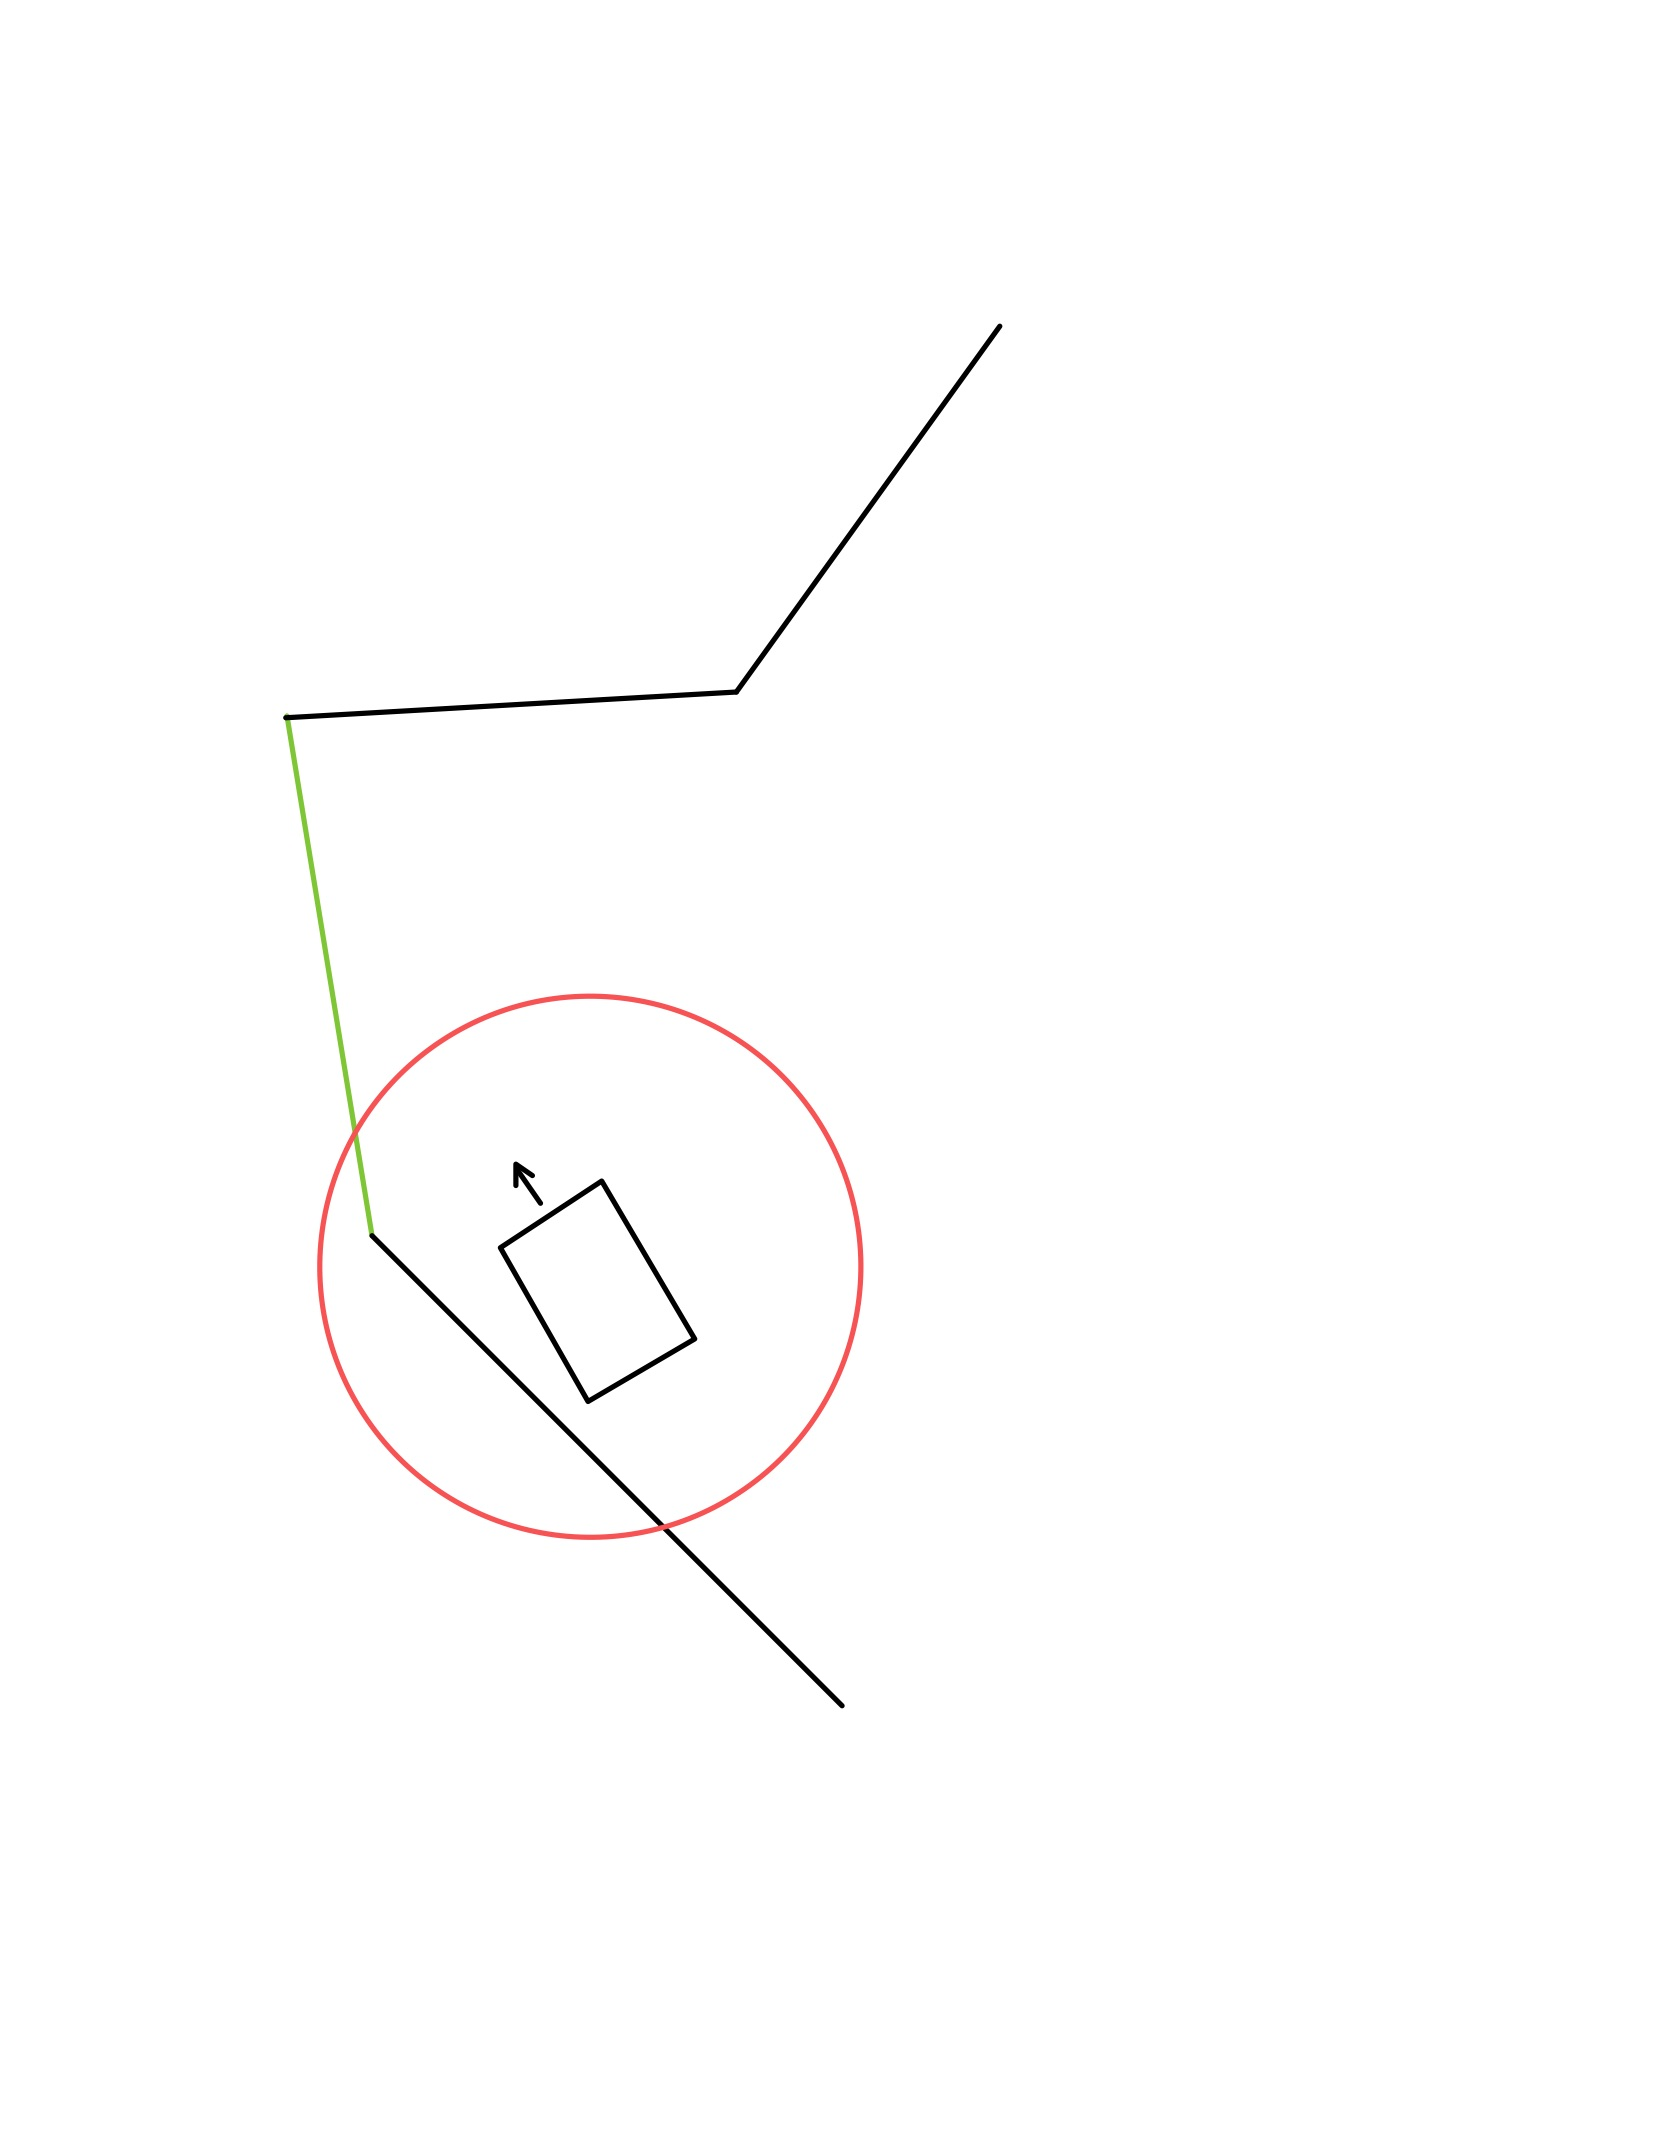
\includegraphics[width=\textwidth]{6.141-53.jpg}
        \caption{Ignore previous segments when finding closest segment}
    \end{subfigure}
    \hfill
    \begin{subfigure}[b]{0.25\textwidth}
        \centering
        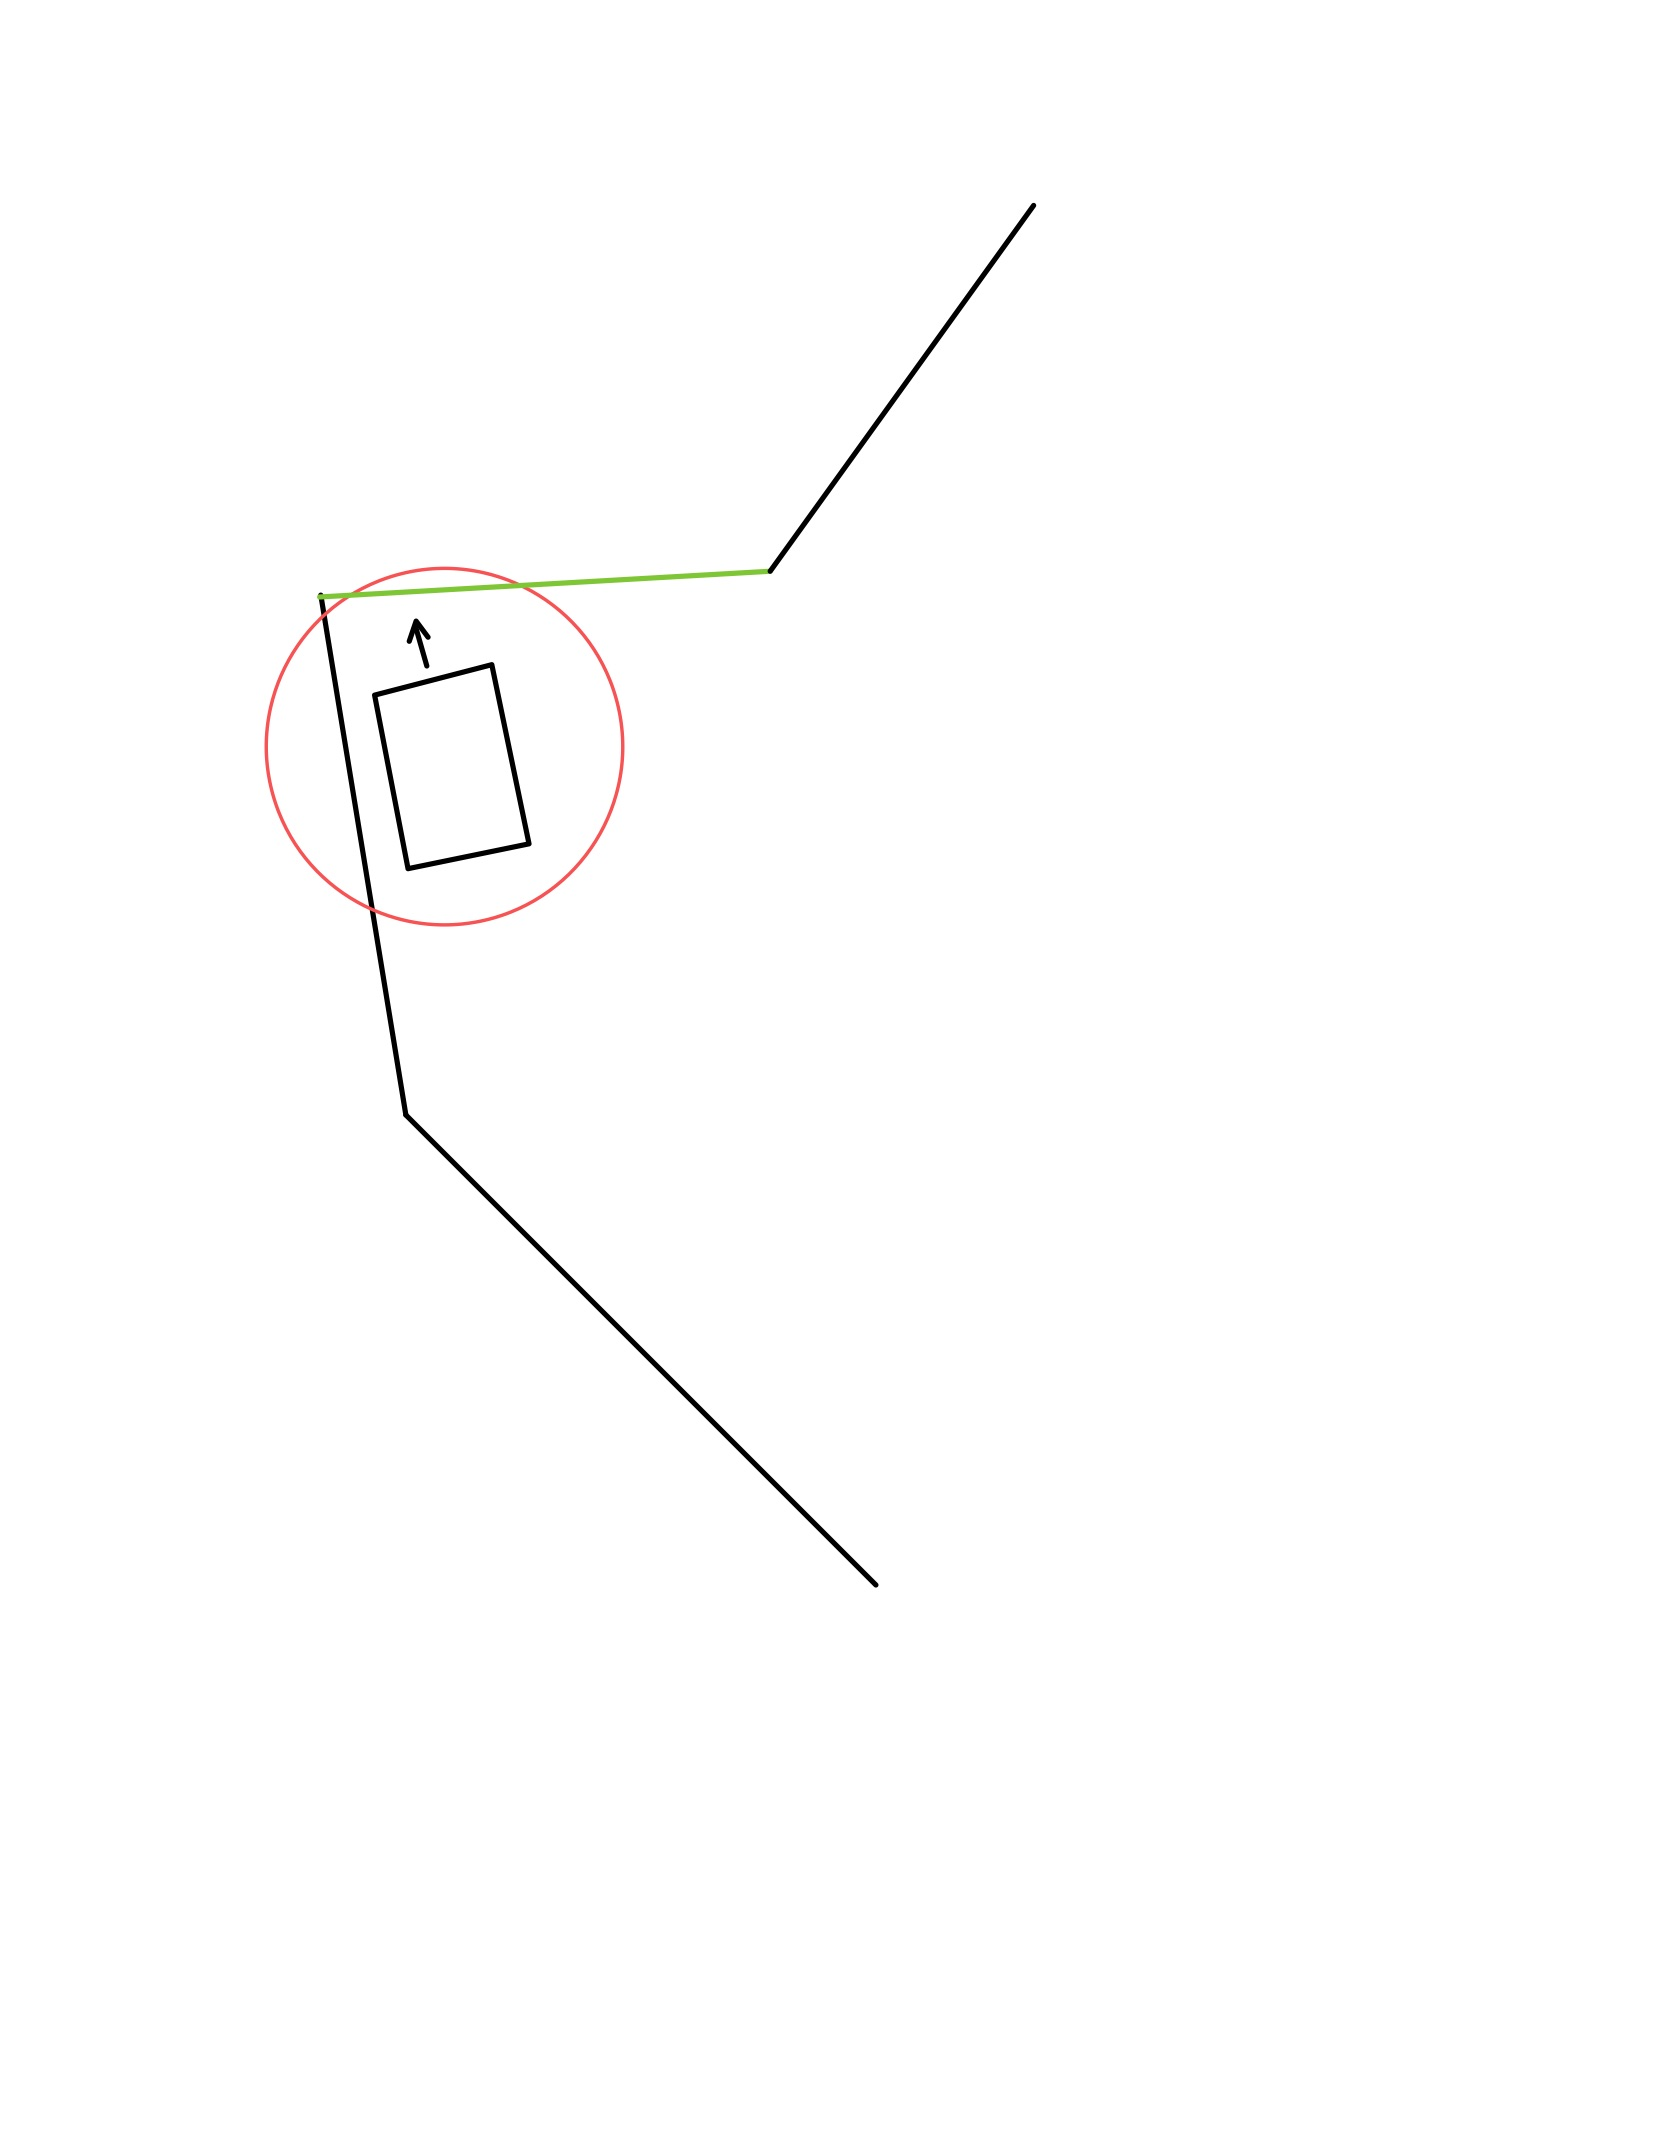
\includegraphics[width=\textwidth]{6.141-54.jpg}
        \caption{Shrink lookahead distance (radius of circle) when encountering high curvature section of path}
    \end{subfigure}
        \caption{Stages of pure pursuit}
        \label{fig:Corner Traversal Figures}
\end{figure}

The minimum distance to the segment is found with Equation 3.

\begin{equation}
    t = max\left(0, min\left( 1, \frac{(point - start) \cdot (end - start)}{12} \right)\right)
\end{equation}

The distance is clamped between 0 and 1 to only include points inside the vector end - start.\\

The projection calculation is shown in Equation 4.

\begin{equation}
    projection = start + t \cdot (end - start)
\end{equation}

Then, the shortest distance is the euclidean distance between the robot's location and and the projection. This is computed for every segment, and the smallest of them corresponds to the closest segment to the robot. We only look at the path ahead of this segment to focus on moving forward. The default target point is the endpoint of the closest segment, but we show how we more completely calculate the target point in Section 2.3.3.

\subsubsection{Determining lookahead distance}

We surround the robot in a bounding circle with radius = lookahead\_dist. When the bounding circle intersects with a segment, the point at which it intersects is the target point.\\



We choose the lookahead\_dist (the radius of a circle) based on the angle between the robot's current location and the desired\_point. In our experiments, we found that one universal constant does not work for trajectories that mix together sharp turns and wide straight paths. \\

Figures 4b and 4c show situations in which the lookahead distance changes based on the curvature of the path. We use a smaller lookahead\_dist (0.5m) if the trajectory within the circle has no angles of greater than 30 degrees. This helps the robot from switching to the next segment too early and accidentally cutting a corner. However, we use a larger lookahead\_dist (1.5m) on low curvature sections to move forward in the path efficiently, without the danger of colliding with a wall.\\

\subsubsection{Calculating target point}

We need to figure out where a line segment intersects a circle, and determine which intersection point to track. For figuring out intersection points, we look at all line segments along the path and figure out where the line extending from those segments intersects the circle. If this point is within the bounds of the segment, we mark an intersection point as found. Once we have figured out the intersection points, we set the one that is furthest along the path as the desired point.\\

We calculate the target point by Equation 5.
\begin{equation}
    \text{target\_point} = \text{start} + t \cdot V
\end{equation}

where V = end - start and t is \_\_, again clamping the result to be within 0 and 1. 

\\We solve t with Equation 6, where $a = V \cdot V$ and $b = 2 \cdot V \cdot \text{(start - point)}$.

\begin{equation}
    t = max\left(0, min\left(1, \frac{-b}{2a}\right)\right)
\end{equation}


\subsubsection{Calculating steering angle}
Finally, we determine the steering angle. The steering angle is calculated using the Ackermann bicycle model, which treats the robot like a bike where the front wheels move together, but separately from the back wheels. This calculation is shown in Equation 7.
 
\begin{equation}
    \text{steering\_angle} = \tan^{-1} \left( \frac{2*\text{wheelbase\_length} \cdot \sin {(\eta)}}  {\text{lookahead\_dist}} \right)
\end{equation}

where $\eta$ is new\_yaw - prev\_yaw\\

\begin{figure}[h]
\begin{center}
    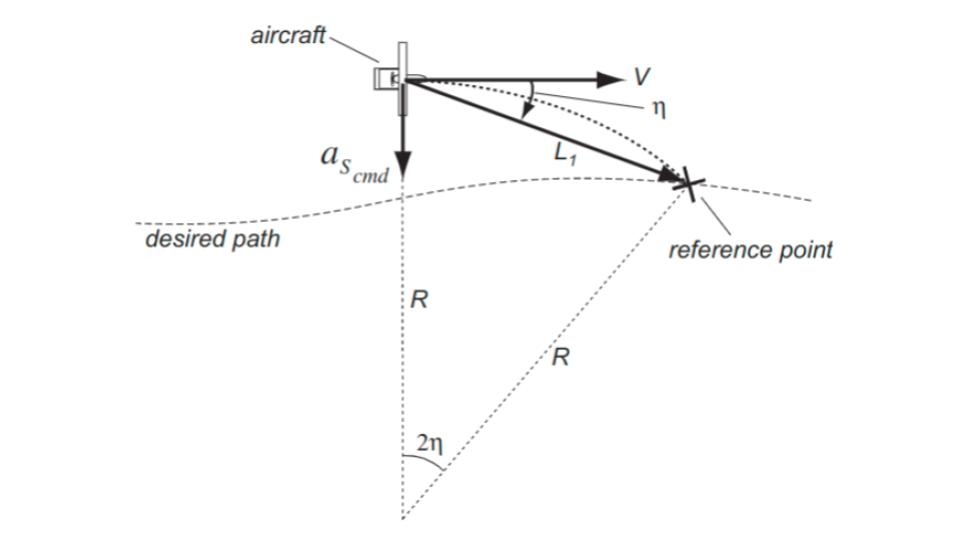
\includegraphics[width=0.5\textwidth]{pure_pursuit_diagram.jpg}
    \caption{The steering angle is calculated as a function of the yaw ($\eta$), wheelbase length, and lookahead distance (R).}
\end{center}
\end{figure}

We publish an AckermannDriveStamped message with the steering angle set, allowing the robot to follow the path with pure pursuit.


\section{Experimental Evaluation}

We may have successfully integrated our path planning algorithm and pure pursuit controller together in simulation, but that was not the end. Evaluation of the performance of our current implementations was essential to brainstorm for possible improvements.

\subsection{Pure Pursuit Controller Evaluation}
Written By: Zoe Wong\\

To determine the performance and robustness of our pure pursuit controller, we decided to measure the error when traveling different paths and different speeds in the Stata basement to analyze how it is affected by the path and speed travelled. 

\subsubsection{Error Collection and Visualization}

We defined error as the Euclidean distance between the real position of the robot and the closest point on the trajectory. Based on this definition, error is greatly dependent on the performance of the localization module, responsible for predicting our current pose, and the pure pursuit controller, responsible for controlling the path travelled the robot. Moreover, as it was difficult to measure the robot’s real position in real-life, we only computed error in simulation.\\

First, to get the ground truth position of the robot in simulation, we listened to the transformation between \texttt{/map} and \texttt{/base\_link}. \texttt{/map} and \texttt{/base\_link} refer to the reference frames of the map center and the robot, respectively. Thus, the translation between these two frames corresponds to the real position of the robot. \\

Given the robot's real pose as computed above, we did not need to find the exact point on the trajectory closest to the robot to measure error. Instead, we simply measured the minimum distance, or the perpendicular distance, between the robot and the trajectory segment the robot was going towards in the previous iteration of the pure pursuit controller. During each iteration of the pure pursuit controller, the robot drove towards a new lookahead point, defined as an intersection between the trajectory and the bounding circle with radius of lookahead distance centered around the robot. Based on this, we can conclude that the robot was likely following the trajectory segment containing the previous lookahead point. Thus, we can focus on this small section of the trajectory, and define the error as the perpendicular distance between this segment and the robot. We computed this distance using the same equation used in the pure pursuit controller to find the closest segment to the robot. \\

This error was published through topic \texttt{/error} at every iteration of the pure pursuit controller when the robot was moving, and recorded as rosbags and .txt files. Afterwards, using the python library \texttt{matplotlib}, we graphed error versus pure pursuit controller iteration to get the plots found in the next section. \\

With these error calculations running in the background, we had the robot travel along the following 3 paths of different lengths and turns, found in Figure 6, at the same speed of 2m/s to measure how error changes depending on the path taken. Additionally, we had the robot repeatedly travel from and to the same pair of start and goal points as Path 2 at different speeds (1m/s, 2m/s, 3m/s, 4m/s) to see if error can be minimized. 

\begin{figure}[h]
\begin{center}
\begin{tabular}{c|c|c}
    Path 1 & Path 2 & Path 3 \\
    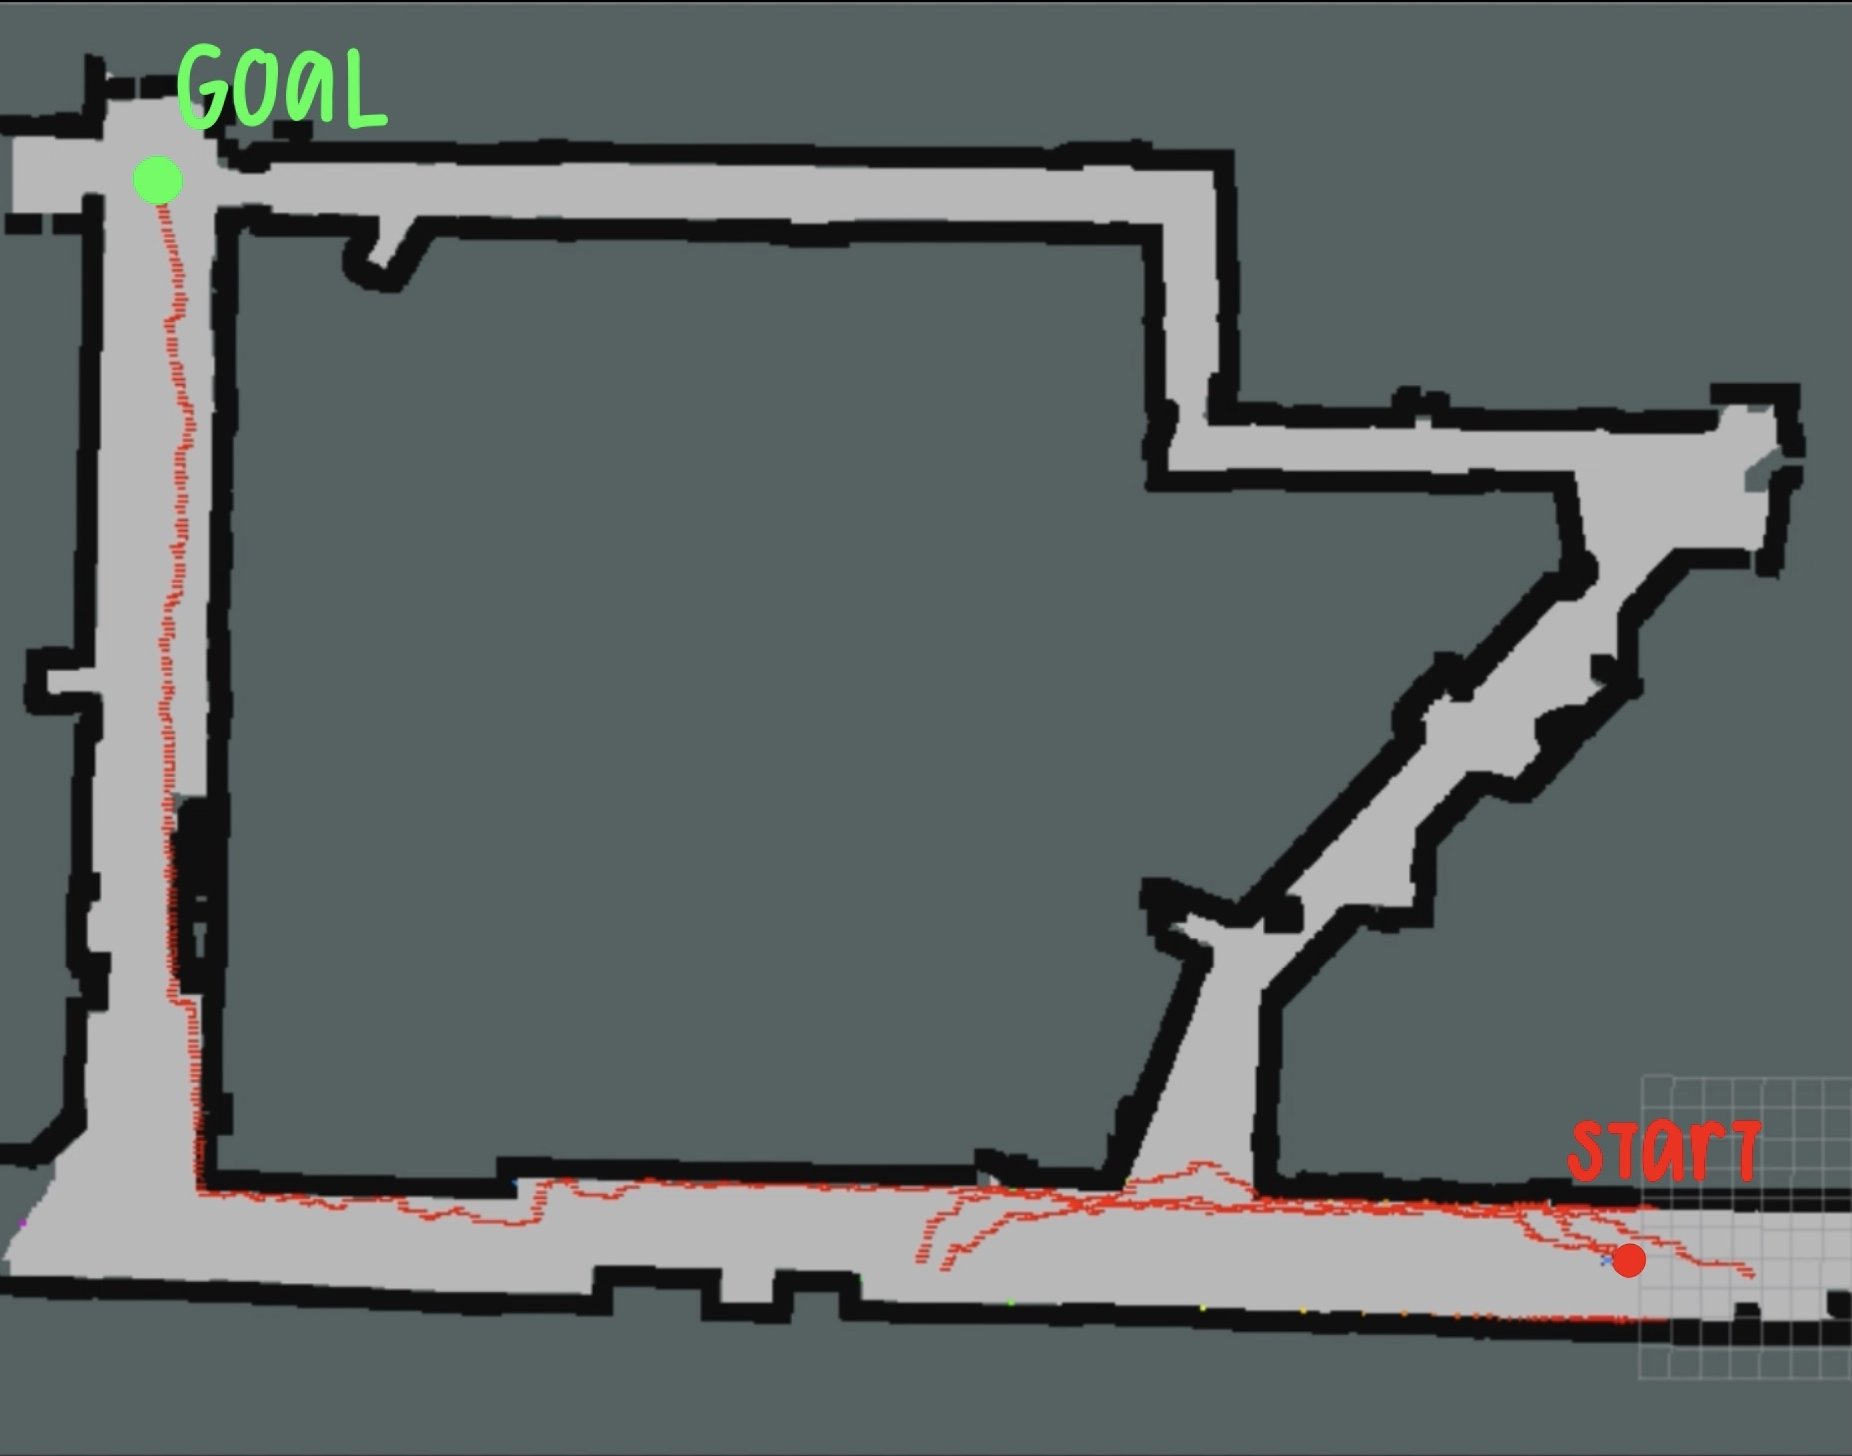
\includegraphics[scale=.08]{path1.png} & 
    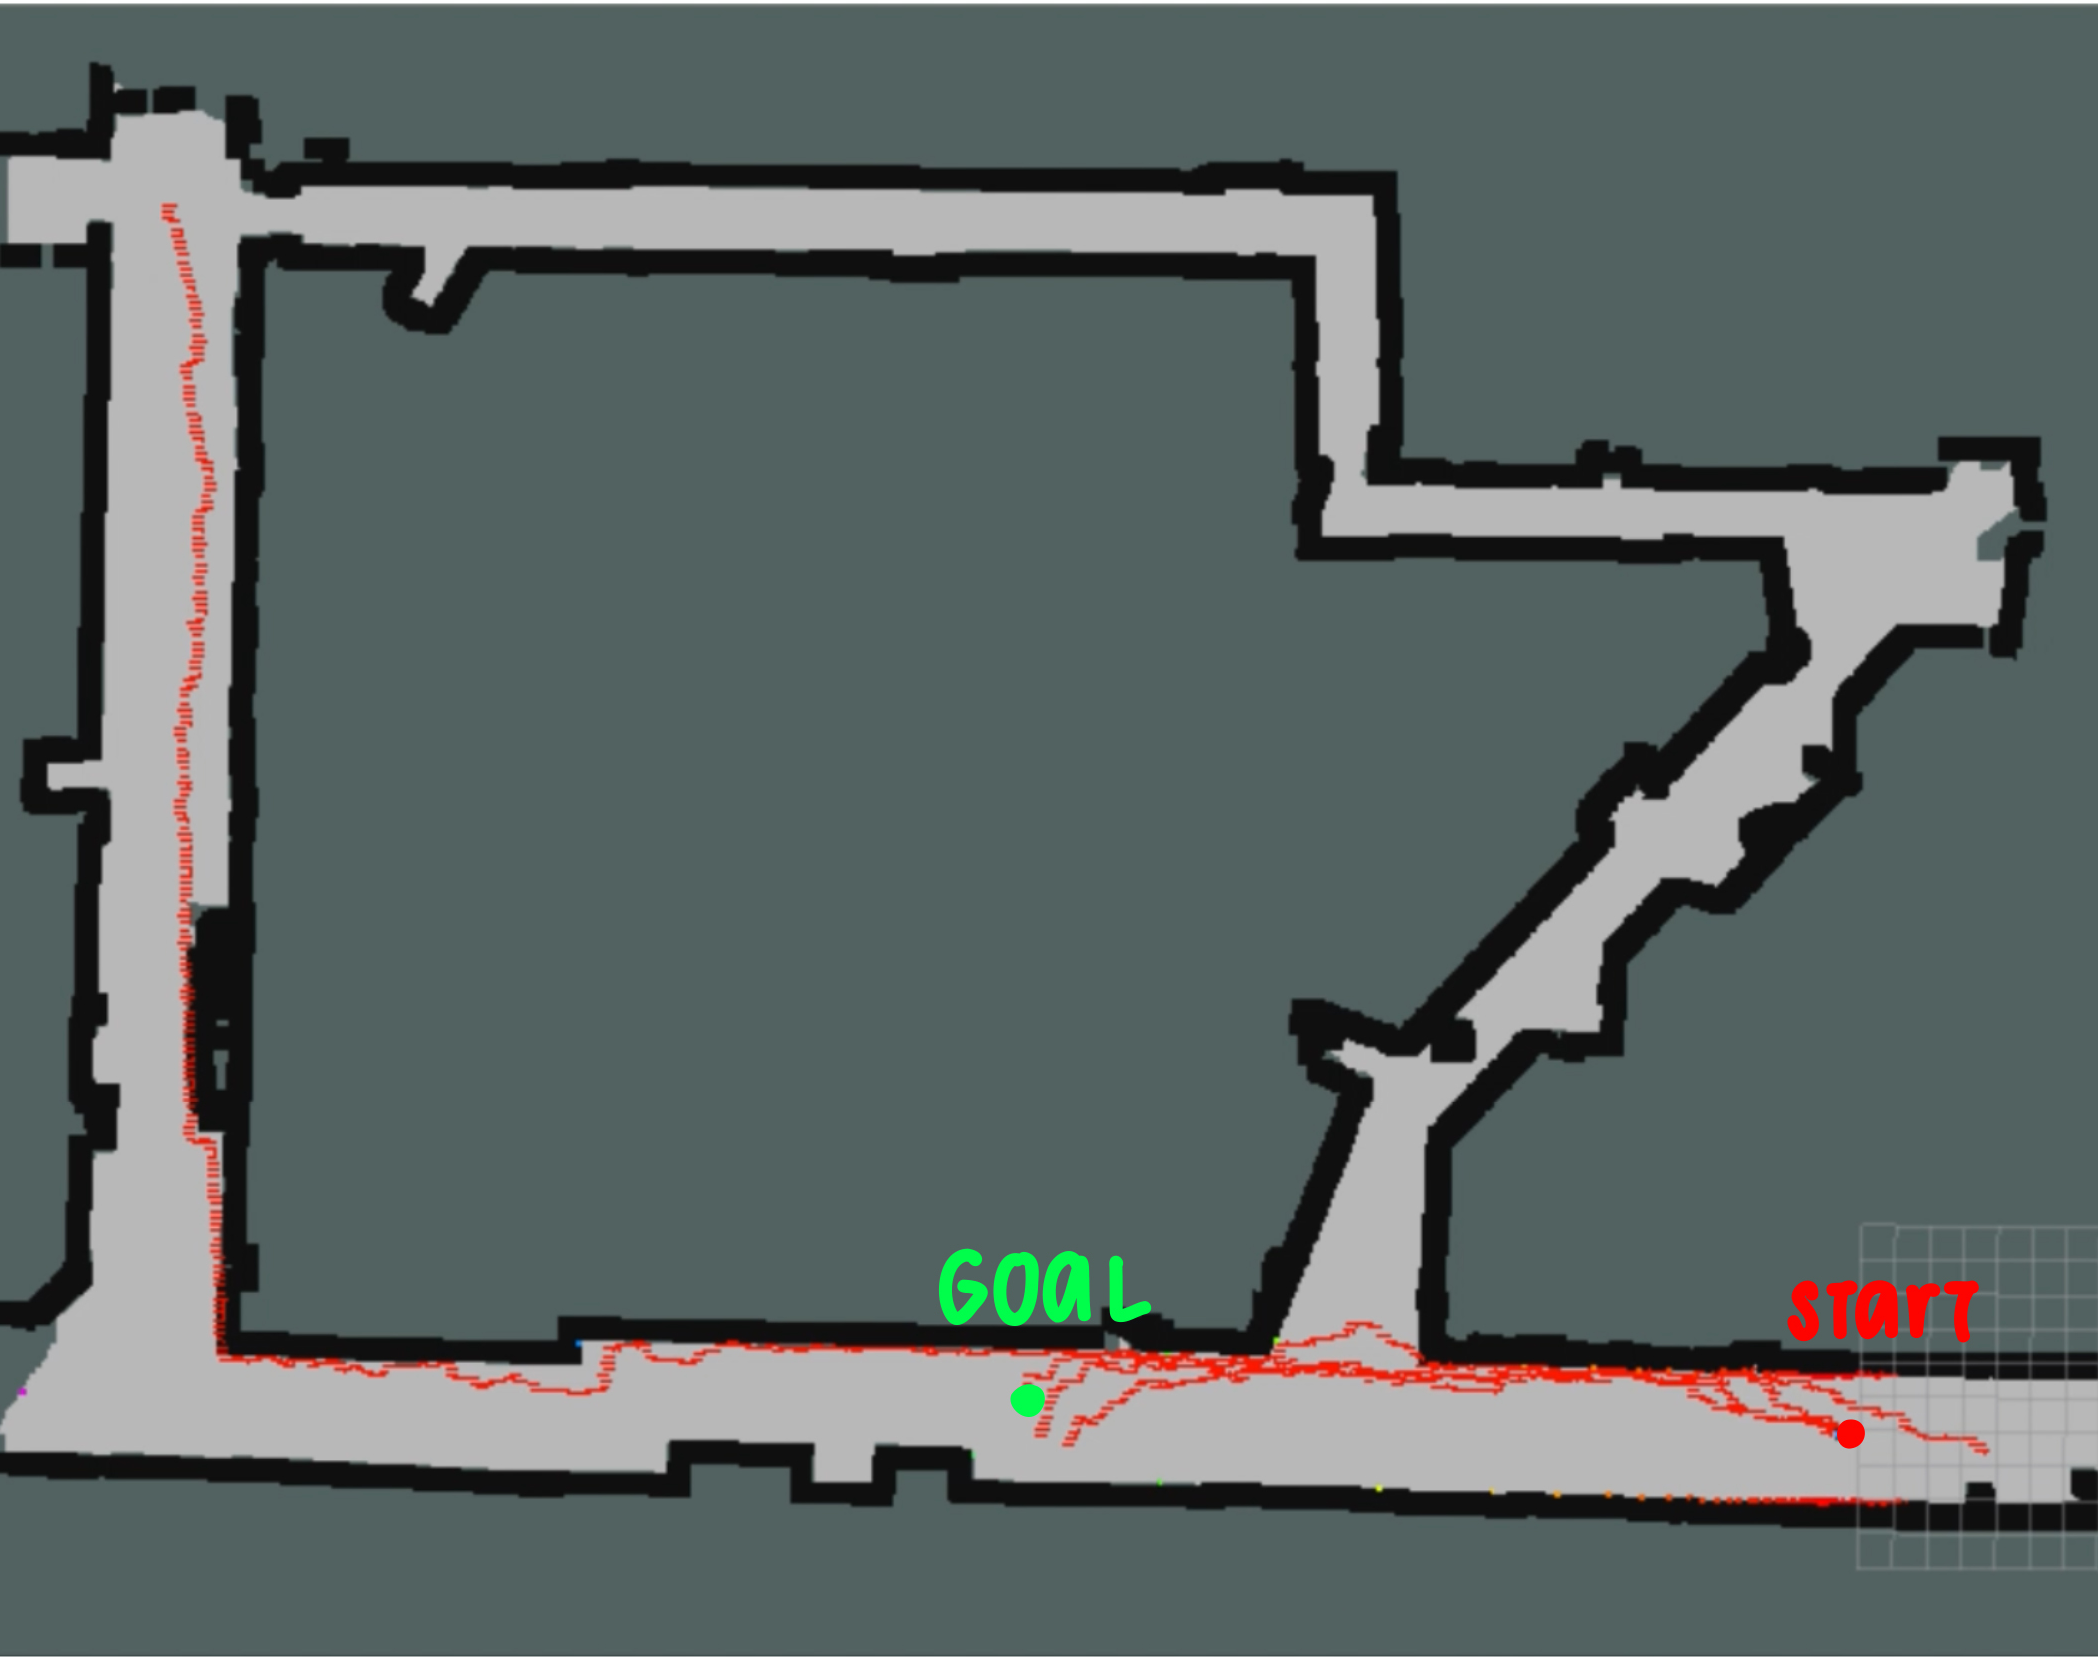
\includegraphics[scale=.07]{path2.png} & 
    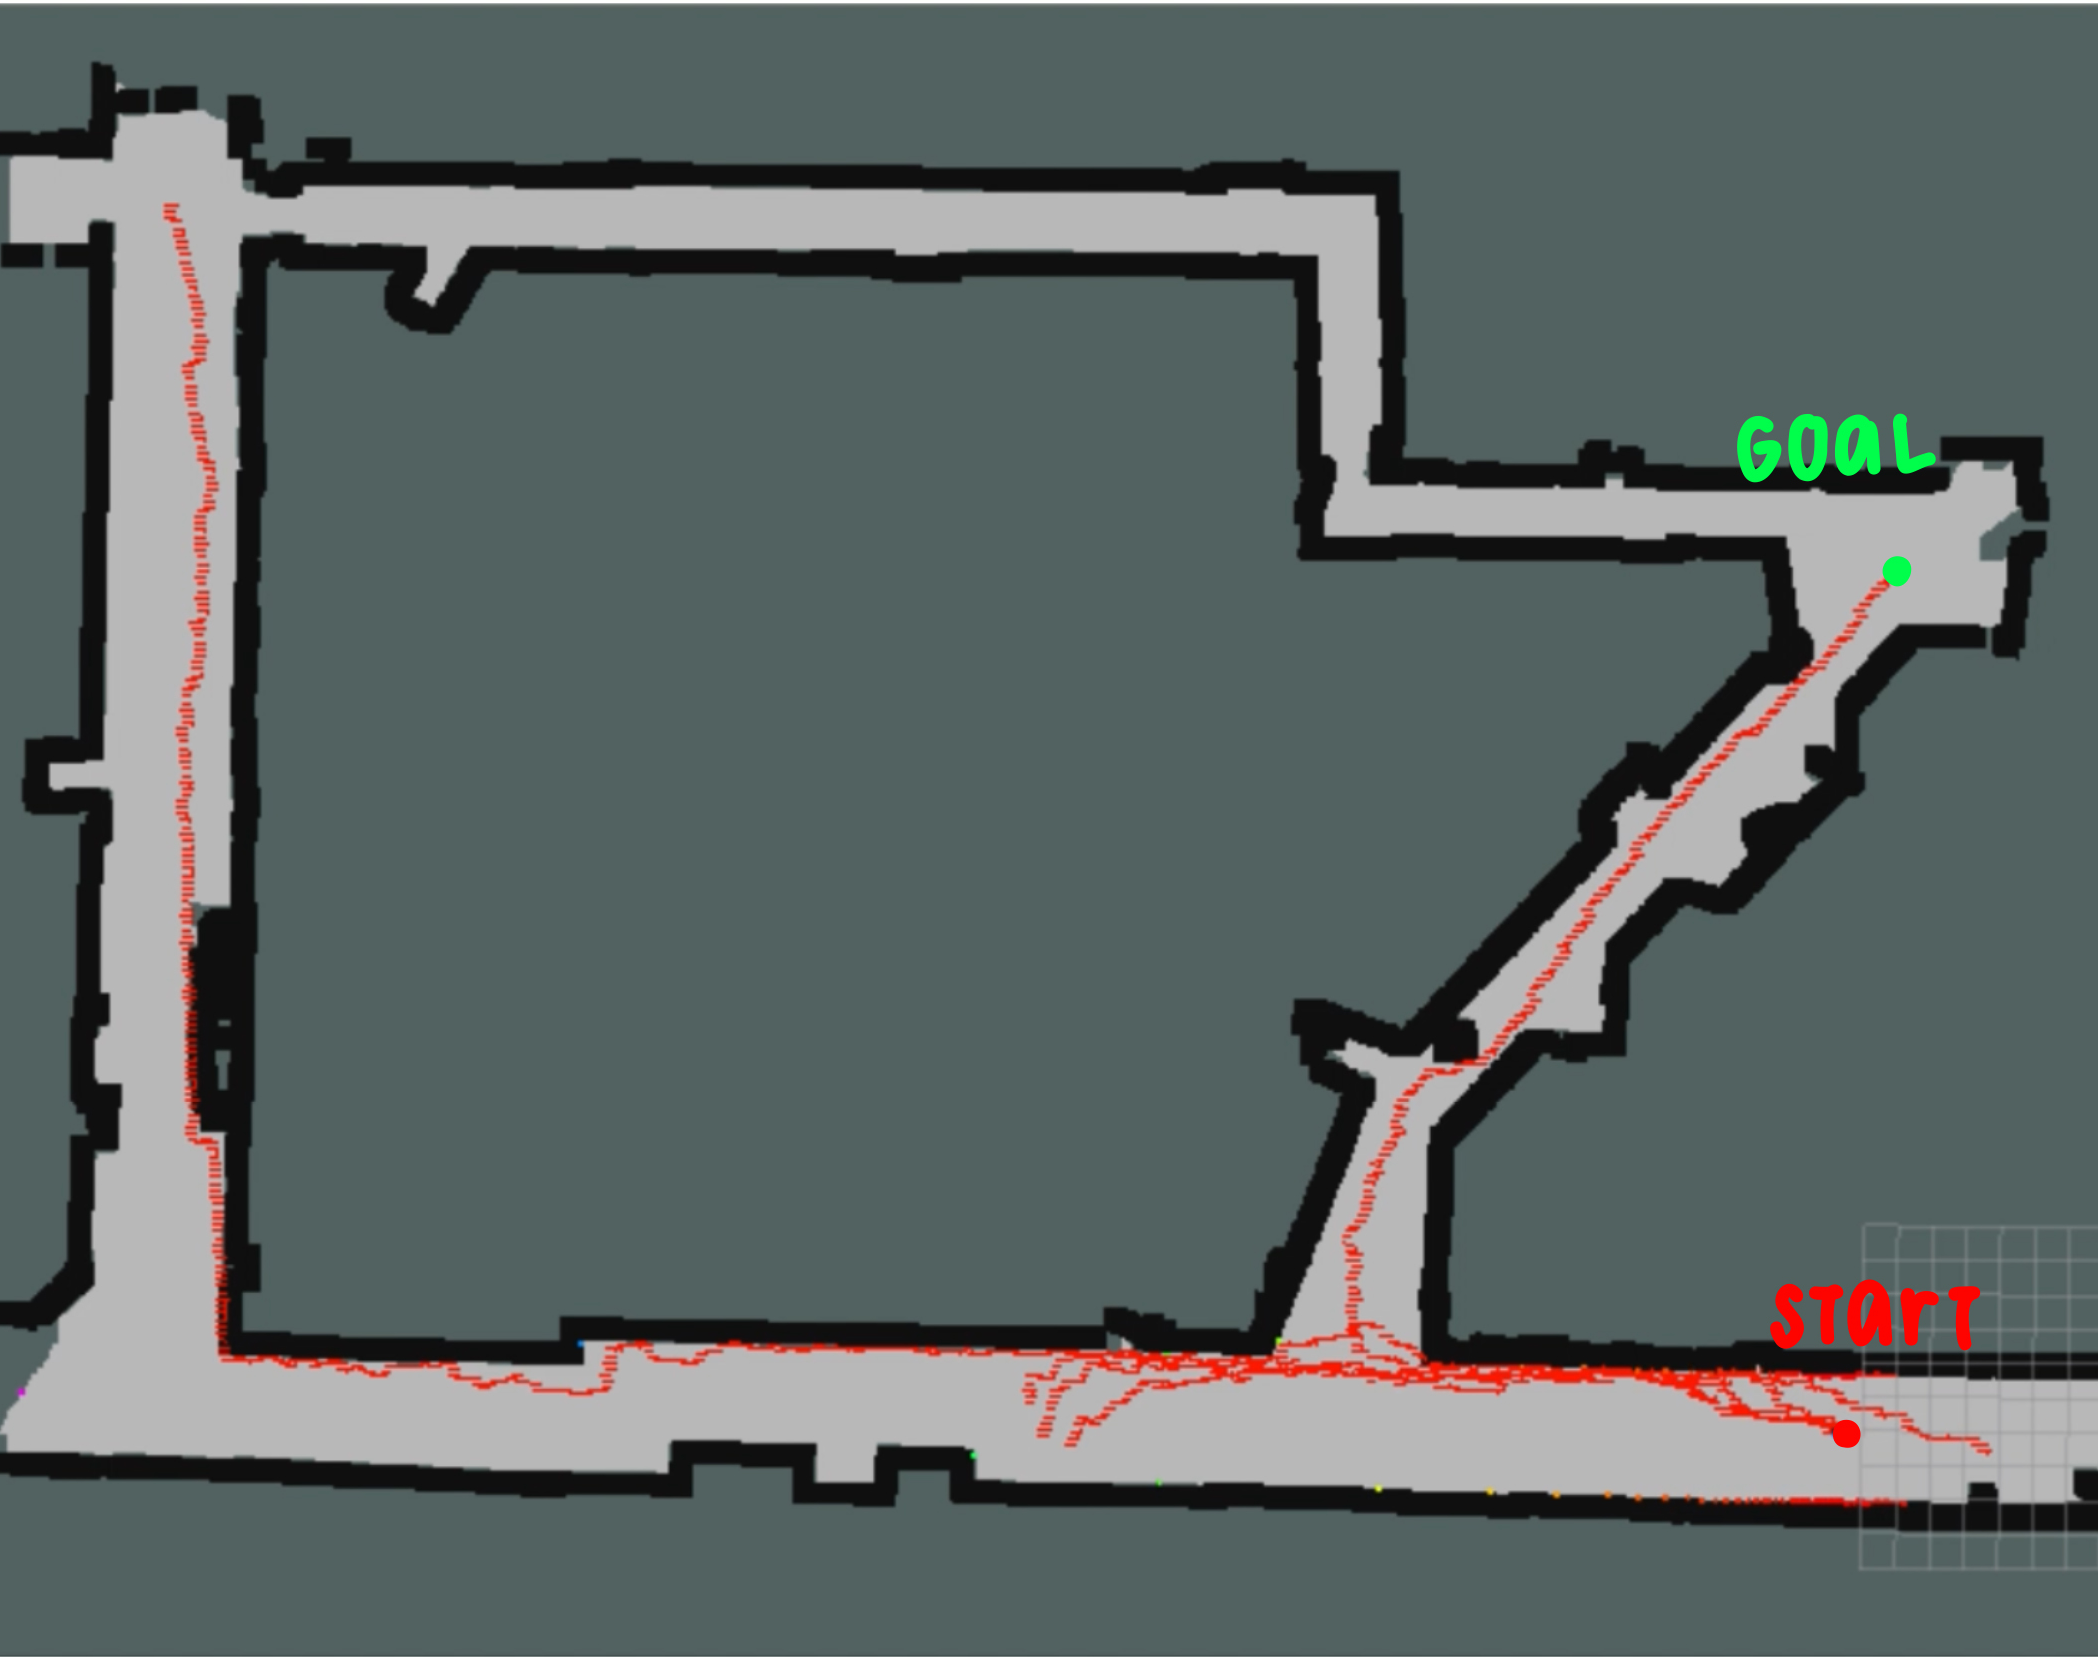
\includegraphics[scale=.07]{path3.png} 
\end{tabular}
\caption{Different Paths Travelled in Simulation to Measure Pure Pursuit Controller Error}
\end{center}
\end{figure}

\subsubsection{Error Analysis}

In Figure 7, we have the error plots (Error versus Pure Pursuit Controller Iteration) for when the robot travels 2m/s along the 3 different paths. First, looking at the error plot for Path 2 (Figure 7b), we could see that the average error along this path was very small (.07 meters, or 7 centimeters), indicating that our pure pursuit controller was decent when travelling a relatively straight and short trajectory. Additionally, the small peaks in the error plot correspond to moments when the robot overshoots the desired trajectory and thus, the error spikes. \\

Now, if we examine the error as the robot is travelling along Path 3 (Figure 7c), we can see that the average error increases to 0.09 meters. This increase in error was due to the large error peaks corresponding to when the robot turns around corners, which makes sense because the robot was still adjusting its orientation during these moments. This conclusion was further supported when we looked at the error plot for Path 1 (Figure 7a). Despite being a much longer trajectory, the average error was approximately the same. This observation indicates that the error when traveling the straighter segments was minimal and thus, did not contribute as much as the error when making the 90 degree turn, supporting the conclusion that error increases around corners.\\

\begin{figure}[h]
\begin{center}
\begin{tabular}{c|c|c}
    (a) Path 1 & (b) Path 2 & (c) Path 3 \\
    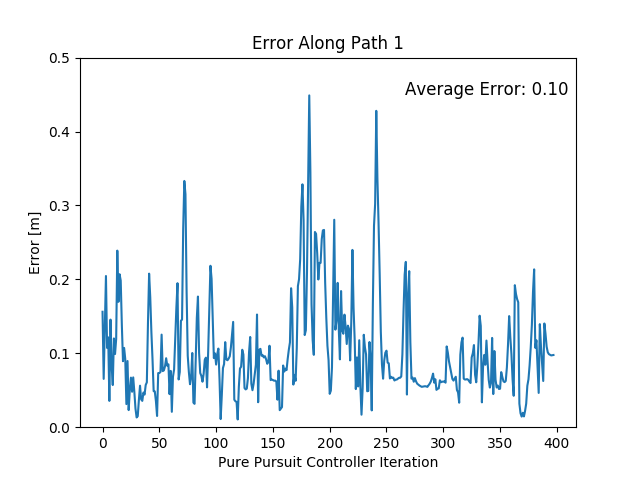
\includegraphics[scale=.33]{path1_error.png} & 
    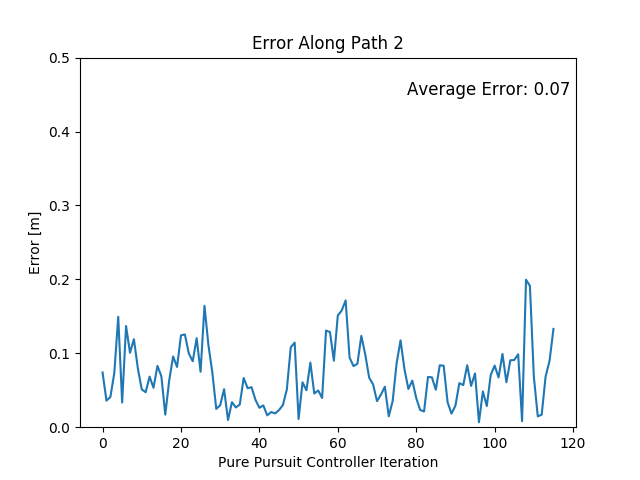
\includegraphics[scale=.33]{path2_error.png} & 
    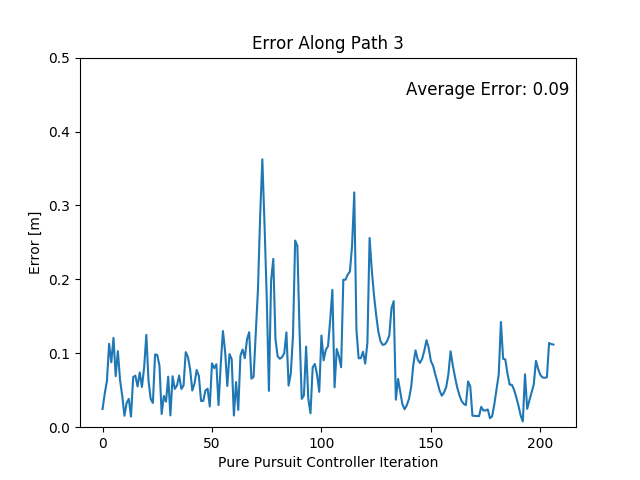
\includegraphics[scale=.33]{path3_error.png} 
\end{tabular}
\caption{Error Versus Iteration Per Path Travelled at Speed=2m/s}
\end{center}
\end{figure}

In Figure 8, we have similar error plots for when the robot is travelling different speeds along paths similar to Path 2 in that they share same pair of starting and ending points. Interestingly, the error rises whether we increase or decrease the speed the robot travels. The average error at 1m/s, 3m/s, and 4m/s were 0.14, 0.14, and 0.13 meters, respectively; all which were greater than the average error when travelling 2m/s (0.07 meters). One potential explanation for why the error was greater when travelling at 1m/s was that the robot does not react as fast when trying to veer back on course. Thus, the robot stays off course for a longer period of time. An explanation for why the error was greater at faster speeds was that the robot tends to overshoot the trajectory since there are less moments for it to adjust to the trajectory because it is moving faster.

\begin{comment}
Additionally, with a small step size used in the RRT algorithm for path planning, the robot would try to follow the trajectory as exact as possible. Therefore, possibly 
\end{comment}


\begin{figure}[h]
\begin{center}
\begin{tabular}{c|c}
    (a) Speed = 1m/s & (b) Speed = 2m/s \\
    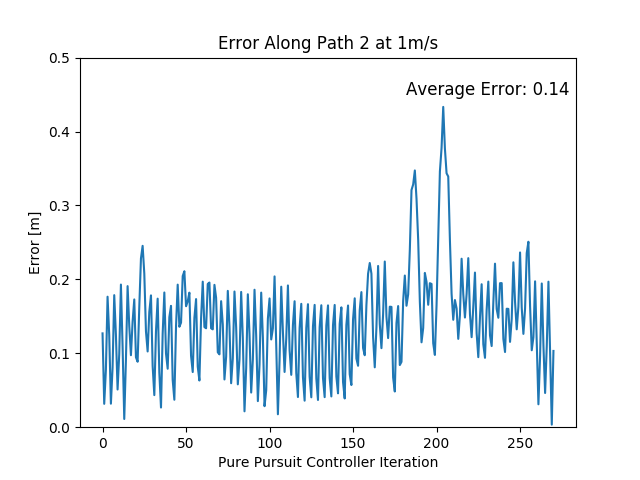
\includegraphics[scale=.5]{path2_speed1_error.png} & 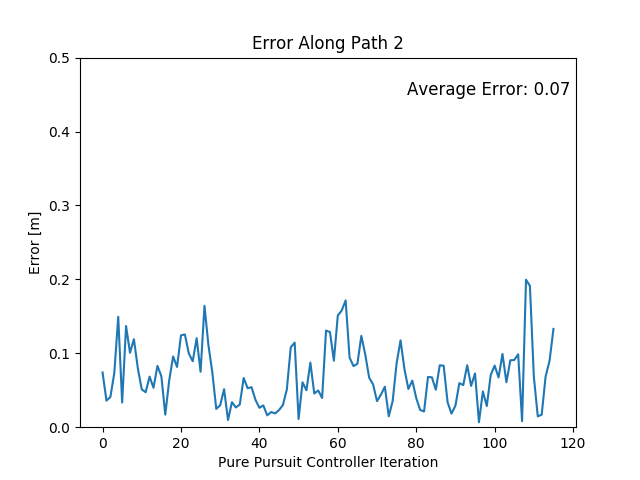
\includegraphics[scale=.5]{path2_error.png} \\
    \hline \\
    (c) Speed = 3m/s & (d) Speed = 4m/s \\
    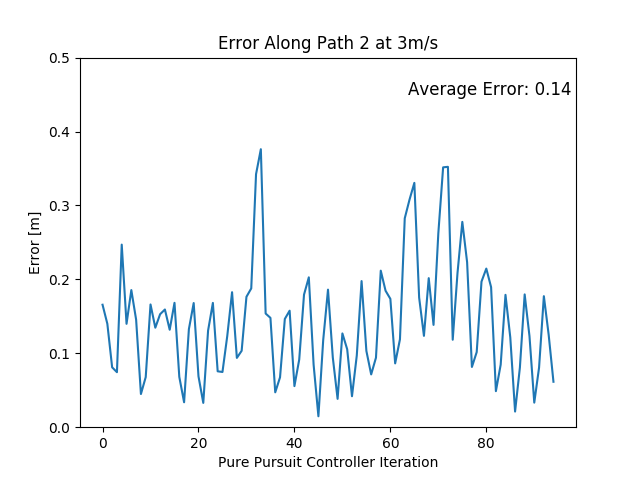
\includegraphics[scale=.5]{path2_speed3_error.png} & 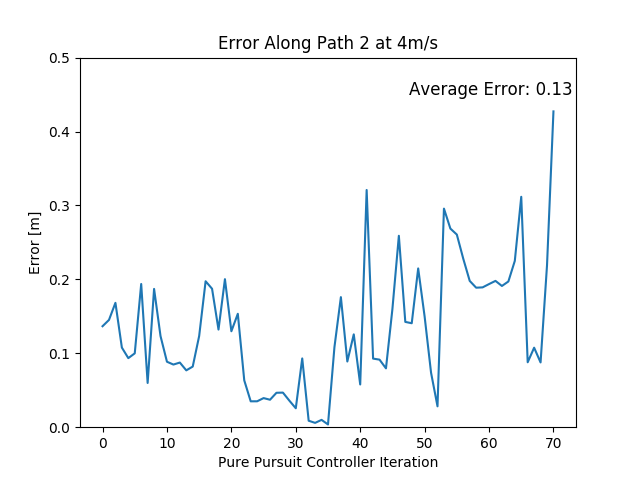
\includegraphics[scale=.5]{path2_speed4_error.png} \\
\end{tabular}
\caption{Error Versus Iteration When Travelling at Different Speeds Along Path 2}
\end{center}
\end{figure}

\begin{comment}
The purpose of this section is to \textbf{provide evidence of the functionality} of your design, and to \textbf{document your experimental evaluation}. The section should explain both:

\begin{enumerate}
\begin{item}
\textbf{what} was tested and \textbf{why}, and \textbf{how} those tests were performed (Technical Procedures, including a clear definition of the performance metrics used in the analysis),
\end{item}
\begin{item}
and \textbf{discuss the result} of those tests to arrive at an assessment of the functionalities you implemented in this lab (Results).
\end{item}
\end{enumerate}

\textbf{You can find ideas and suggestions in the “Good Experimental Evaluation” Recitation on Canvas (Modules section).}\\\\
(no more than 1250 words)

\end{comment}

\subsection{Real Life Car Implementation}
Written by: Frank Gonzalez\\ 

In order to transfer path planning and pure pursuit onto the real life car, we needed a functional localization package so that the car could track itself as it moved along the planned trajectory. Unfortunately, the localization package we used experienced divergence when run in conjunction with path planning and pure pursuit. With more allotted time, we would work towards properly synthesizing the two packages to conduct a proper test of our algorithm in real life.

\section{Conclusion}
Written by: Toomas Tennisberg\\\\
The racecar is capable of eventually finding and following a path to a given destination. RRT's convergence time is highly variable on the path ranging from a few seconds to around a minute. A* however, is consistent and scales with path length while remaining relatively low. Pure Pursuit successfully follows the given path without crashing into a wall. Therefore, we believe our car is capable of autonomous navigation within the real world.\\
\pagebreak

\section{Lessons Learned}
\subsection{Frank Gonzalez}
On the techical side, I got more familiarity with implementing search algorithms like RRT and A*, and I learned about the importance of visualizing your algorithm in order to debug it. I ran into some very nuanced bugs regarding how numpy matrices worked, and if I hadn't visualized my trees or the obstacle calculations, I wouldn't have ever found my bugs. In addition to abstract path planning, I had the liberty of choosing some fun representations for the trees and algorithms.\\

On the communications side, I learned how to better communicate why certain goals weren't met and the setbacks that both I and the team experienced while trying to accomplish some of our goals, which I now believe to be just as important as communicating the successes. 

\subsection{Marisa Hoosen}
This lab, I got more practice implementing math for pure pursuit and debugging. I reviewed more of the geometry used in controlling the car, and got more familiar with the bike model.\\

In the communication aspect, I got more practice writing the explanation of the algorithm rather than the evaluation. I've improved more with fitting the information I present to fit within a given time frame, and determining what is most relevant of the information needed to present.\\

I worked with others on pure pursuit this lab moreso than other labs. We worked side by side nearly the entire time, and bounced ideas off each other to get the code working. 


\subsection{Toomas Tennisberg}
I found helping out with figuring out why our Pure Pursuit implementation was not working a really useful experience in debugging code and asking for help from people. The behaviour of the system was extremely confusing at one point and I am still not entirely sure what was causing it.\\\\
On the CI side, I learned that I am terrible at doing work when I'm all alone and don't have social peer pressure to push me into contributing. Therefore, I believe that I should be more proactive about calling for team meetings and working on the task at hand.

\subsection{Zoe Wong}

On the technical side, this lab helped me review the essential geometry when trying to implement the pure pursuit controller to find the closest trajectory segment and when finding bounding circle intersections. Additionally, since, depending on the step size used in the RRT algorithm for path planning, the number of trajectory segments is changes, we had to be efficient with how we were computing the minimum distances between the robot and all of the segments to minimize runtime. For this reason, I gained a lot of experience and practice with using the python library numpy to vectorize functions so that they could be called in parallel.\\

In the communication and collaboration aspect, this lab also helped me realize the importance of asking for help and conveying my confusions and questions to others, including my peers and the TAs. In the beginning, when I just started implementing the pure pursuit controller, I was quite confused with the importance of finding the closest segment when we only needed to find and determine the next lookahead point. However, after receiving help from a TA, it all made sense and this understanding helped a lot with future debugging because I knew what the algorithm needed to do to work successfully. Additionally, while working on the pure pursuit controller, I had some trouble sending the right drive commands to the robot as it would always veer off course. With help from my team members, we were able to decipher the problem and debug the code to get it to work properly!\\


\begin{comment}
1. technical side: debugging for pure pursuit controller, review of geometry, decrease runtime\\ 
2. communication: concise with words and conclusion during briefing, especially if short on time \\
3. collaboration: collaboration on pure pursuit module to make sure work as whole together\\
\end{comment}

\subsection{Kaitlin Zareno}
On the technical side, I learned how to implement RRT and now better understand the differences between RRT and A* in different situations. Before this class, I had never encountered RRT, so it was cool to learn about this new concept in lecture and apply it on our robot. I also learned about the importance of visualizations in debugging; earlier on in the semester, visualizations were a bit tedious and seemed unnecessary, but now they were extremely helpful towards recognizing if our search algorithms were progressing in ways that seemed logical, and determining how to best fix the bug at hand. I'm sure that being good about making and analyzing our visualizations of our algorithms will come in handy during the final challenge. \\

On the CI side, I learned how to stay more calm when answering Q&A questions during the briefing. I had been dreading answering Q&A questions the entire semester; when I get nervous, I lose the ability to fully regulate my thoughts and reactions, and these feelings are particularly heightened in the Q&A when I feel less than 100 percent confident in my ability to "jump in" and sound coherent and credible. In order to combat these heightened feelings, I've been working on trying to take a step back and work through my thoughts in these moments of panic, and I think I've made progress towards being more calm and confident in stressful situations. 

\begin{comment}
\section{Formatting examples for figures, pseudocode, etc}

\subsection{Tables}

Many other table packages and options exist but here is one example:\\\\

\begin{tabularx}{0.8\textwidth} {
  | >{\raggedright\arraybackslash}X
  | >{\centering\arraybackslash}X
  | >{\raggedleft\arraybackslash}X | }
 \hline
 item 11 & item 12 & item 13 \\
 \hline
 item 21  & item 22  & item 23  \\
\hline
\end{tabularx}

\subsection{Images}

\begin{figure}[h]
\begin{center}
\includegraphics[width=0.65\textwidth]{placeholder} % Include the image placeholder.png
\caption{Figure caption.}
\end{center}
\end{figure}

\subsection{Code Blocks and Algorithm Pseudocode}

% Including Python code blocks:

\begin{lstlisting}
json
{
  "6.141": "normal",
  "16.405": "woke",
  "no_sleep": "spoke"
}

def do_something_productive():
  if not_productive:
    do_work()
  else:
    cry()
\end{lstlisting}

% Using the algorithm2e package for pseudocode:

\begin{algorithm}[H]
\SetAlgoLined
 \While{alive}{
  \eIf{sleepy}{
   sleep\;
   }{
   eat\;
  }
 }
 \caption{caption}
\end{algorithm}

% Using the algorithmic package for pseudocode:

\begin{algorithmic}
\STATE $i\gets 10$
\IF {$i\geq 5$}
        \STATE $i\gets i-1$
\ELSE
        \IF {$i\leq 3$}
                \STATE $i\gets i+2$
        \ENDIF
\ENDIF
\end{algorithmic}
\end{comment}

\end{document}